
\documentclass[11pt,a4paper]{article}
\usepackage[margin=1in]{geometry}
\usepackage{amsmath,amssymb}
\usepackage{booktabs}
\usepackage{array}
\usepackage{hyperref}
\usepackage{float}
\usepackage{xcolor}
\usepackage{graphicx}
\usepackage{caption}
\usepackage{microtype}
\usepackage{enumitem}
\usepackage{fancyhdr}
\usepackage{url}
\usepackage{xurl}
\usepackage{adjustbox}
\usepackage{tikz}
\usepackage{pgfplots}
\usetikzlibrary{arrows.meta,positioning,fit,backgrounds}
\usepgfplotslibrary{fillbetween}
\pgfplotsset{compat=1.18}

\hypersetup{colorlinks=true, linkcolor=blue, urlcolor=blue, citecolor=blue}
\pagestyle{fancy}
\setlength{\headheight}{14pt}
\fancyhf{}
\lhead{Cold OCI Image Caches in Kubernetes CI/CD}
\rhead{Research Model}
\cfoot{\thepage}
\Urlmuskip=0mu plus 1mu

\newcommand{\Prob}{\mathbb{P}}
\newcommand{\E}{\mathbb{E}}

\title{Measuring CI Feedback Delay from Cold OCI Image Caches}
\author{Julian Wachter}
\date{\today}

\begin{document}
\maketitle


\begin{abstract}
Kubernetes-based CI/CD systems can lose node-local OCI image cache state whenever CI nodes are rotated. For GitLab Kubernetes executor workloads, this can delay developer feedback because build, test, helper, or service images must be pulled and prepared again before useful CI work can begin.

This paper models that delay as developer-facing cold-node exposure. The model evaluates one OCI image \(I\) at a time, separates jobs scheduled onto cold nodes from nodes that become newly warm, and converts image-availability waiting into affected job-minutes. The same per-image calculation is then applied to image portfolios, where prewarming becomes a prioritization problem: which images should be made available on which eligible CI nodes before developer-facing CI load arrives?

The paper also describes how the model can be evaluated from real GitLab Kubernetes executor workloads. A day of runner Pods can be replayed from Prometheus, Kubernetes lifecycle timestamps, Events, and GitLab job metadata to reconstruct warm-node state, estimate cold-node exposure after node rotation, and compare counterfactual policies such as no prewarming, paced prewarming, cluster-local mirroring, and combined approaches. Discovery is framed as a query--signal--ranking pipeline, so usage, concurrency, developer-window, and pull-cost signals can be evaluated as explicit prewarming policies. A synthetic evaluator is included as a methodology sanity check; production measurements are required for operational claims.
\end{abstract}

\section{Introduction}

CI/CD systems are part of the developer feedback loop. Developers push changes, wait for builds or tests, and use the resulting feedback to decide whether they can continue, fix a problem, or request review. In Kubernetes-based CI/CD systems, this feedback loop can be delayed before the actual build or test work begins: if a job is scheduled onto a node where the required OCI image is not locally available, the node must first fetch, unpack, or otherwise prepare that image.

The problem becomes especially visible in Kubernetes CI node pools operated with immutable infrastructure. Node rotation can be triggered by security updates, Kubernetes upgrades, operating-system image updates, hardware replacement, or immutable-infrastructure rollouts. In clusters operated in an immutable-infrastructure style, as commonly used with Cluster API, updates are applied by replacing nodes rather than by preserving node-local runtime state in place \cite{clusterapioverview,clusterapiconcepts}. When a node is replaced, its local container image cache is lost.

This paper models the resulting delay as developer-facing cold-node exposure. A cold node-local image cache is not only an infrastructure efficiency problem; it can directly affect developers because CI jobs start later and feedback arrives later. The central distinction is that jobs can be affected faster than nodes become warm. Several jobs may be scheduled onto the same cold node before image availability changes, and all of those jobs may wait, but that node becomes newly warm only once.

The model first considers one OCI image \(I\) at a time. For image \(I\), each eligible CI node is either warm or cold. A node is warm if \(I\) is locally available for the job startup path; otherwise it is cold. The model compares sequential arrival, burst arrival, and rolling concurrency, then converts image-availability waiting into affected job-minutes. This single-image model is the mathematical base for the rest of the paper.

The paper then applies the same calculation to a representative CI node-pool rotation scenario and to a portfolio of CI images. The portfolio view is important because real CI systems use many build, test, helper, service, deployment, and project-specific images. In such systems, prewarming is not simply a question of whether an image cache can be filled. It is a prioritization problem over images, nodes, and time windows.

Finally, the paper turns the model into an evaluation method for GitLab Kubernetes executor workloads. A full day of runner Pods can be reconstructed from Prometheus, Kubernetes lifecycle timestamps, Kubernetes Events, kubelet or runtime metrics, and GitLab job metadata. Replaying that workload makes it possible to estimate the impact of node rotation and compare counterfactual policies such as no prewarming, paced prewarming, cluster-local mirroring, and combined approaches. Drop is used as one reference implementation of automated prewarming, not as a requirement of the model.

This paper contributes a per-image exposure model, a portfolio prioritization method, and a real-cluster replay methodology for GitLab Kubernetes executor workloads. First, it defines a warm-node/cold-node model for Kubernetes-based CI/CD workloads. Second, it separates affected jobs from newly warmed nodes and explains why burst scheduling, sequential arrival, and rolling concurrency differ. Third, it extends the model to image portfolios and usage-based prewarming prioritization. Fourth, it proposes a benchmark and replay methodology for measuring cold-node exposure in real GitLab Kubernetes executor clusters after node rotation.

\section{Per-Image Model Setup}

The model analyzes one OCI image \(I\) at a time. In practice, \(I\) should be interpreted as a concrete image reference, preferably identified by digest rather than by a mutable tag. Examples include a Python test image, a Java build image, or a Docker build image used by CI jobs. For this image \(I\), each eligible CI node is either warm or cold: the node is warm if \(I\) is already locally available for the job startup path, and cold otherwise.

An eligible CI node is a node on which the Kubernetes Pod could be scheduled after the usual cluster and runner constraints are applied, such as node selectors, taints and tolerations, resource requests, and CI-runner configuration. A node can be warm for one OCI image and cold for another. The portfolio section later repeats the same per-image calculation for multiple images and aggregates the resulting waiting exposure.

The model compares two timing assumptions. In a \emph{sequential} interval, jobs using image \(I\) arrive one after another with enough time between them that a job scheduled onto a cold node can make that node warm before the next job is scheduled. In a \emph{burst interval}, a group of CI job Pods is created close together, such as in a fan-out stage of a CI pipeline. The burst assumption means that jobs in the group are modeled as observing the cache state that existed when the group started.

\begin{table}[H]
\centering
\renewcommand{\arraystretch}{1.12}
\caption{Notation used in the per-image model. The symbols describe one OCI image \(I\).}
\label{tab:notation}
\small
\begin{tabular}{ll}
\toprule
Symbol & Meaning \\
\midrule
\(I\) & OCI image analyzed by the per-image model \\
\(N\) & eligible Kubernetes nodes in the CI node pool \\
\(N_w(I)\) & warm nodes for image \(I\) \\
\(N_c(I)\) & cold nodes for image \(I\) \\
\(c\) & concrete cold-node count for image \(I\) at the start of the modeled interval \\
\(J\) & jobs in a sequential interval \\
\(J_b\) & jobs in one burst \\
\(A_{\mathrm{burst}}(I)\) & affected jobs in a burst: jobs scheduled onto nodes cold for \(I\) at burst start \\
\(A_{\mathrm{seq}}(I)\) & affected jobs under sequential arrival for image \(I\) \\
\(N_{\mathrm{new}}(I)\) & newly warmed nodes: cold nodes that receive at least one job using \(I\) \\
\(M_{\mathrm{burst}}(I)\) & affected job-minutes under burst arrival for image \(I\) \\
\(M_{\mathrm{seq}}(I)\) & affected job-minutes under sequential arrival for image \(I\) \\
\(p_I\) & modeled image-availability time for image \(I\) on a cold node, in seconds \\
\(f(t)\) & developer-time weight for affected minutes at time \(t\) \\
\bottomrule
\end{tabular}
\end{table}

The basic node-state identity is:
\begin{equation}
N_w(I) + N_c(I) = N.
\end{equation}
For one OCI image \(I\), every eligible node is either warm or cold with respect to that image.

The model estimates expected exposure, not measured end-to-end runtime latency. The actual delay of a CI job depends on kubelet behavior, the configured container runtime, registry performance, image layers, shared layer reuse, image garbage collection, and node I/O. The parameter \(p_I\) represents the assumed or measured time until image \(I\) becomes available on a cold node. In a concrete evaluation, \(p_I\) can be a measured mean, a percentile, or a scenario parameter.

The model counts jobs scheduled onto cold nodes separately from image pulls or image-preparation operations. Several jobs may wait on the same cold node while image \(I\) is becoming available, but that does not mean they cause several independent node-local image pulls. This distinction is why the paper separately tracks affected jobs and newly warmed nodes.

An affected job-minute is aggregate waiting exposure. If 10 CI jobs each wait 60 seconds because their nodes are cold for image \(I\), the system creates 10 affected job-minutes. If those jobs wait in parallel, the wall-clock delay may be much lower than 10 minutes, but the aggregate CI feedback exposure across jobs is still 10 job-minutes.


\section{Core Per-Image Model}\label{sec:core-model}

\subsection{Scheduling interval and assumptions}

This section derives the per-image expectations for one OCI image \(I\) under the placement baseline. At the start of a modeled scheduling interval, \(c\) of the \(N\) eligible CI nodes are cold for \(I\). A job using \(I\) is counted as affected if it is scheduled onto a node that is cold for \(I\) at the moment relevant to the arrival model.

Unless stated otherwise, the model uses a uniform placement baseline: each job is modeled as being scheduled independently onto one of the \(N\) eligible CI nodes. This is not a claim that the Kubernetes scheduler places Pods uniformly in production. It is a neutral reference model that isolates the effect of cache state and can later be compared with scheduler-locality behavior or measured placement data. Scheduler-aware effects are discussed in Section~\ref{sec:scheduler-notes}.

The model separates two outcomes. Jobs can be exposed to waiting time, and nodes can become warm. A node becomes warm for \(I\) only after the required image pull or preparation has completed on that node. This distinction is the reason prewarming is evaluated both as cache-state progress and as developer waiting exposure.

The small examples in this section use \(N=10\) nodes, \(c=6\) cold nodes for image \(I\), \(J_b=5\) jobs in one burst, and \(p_I=60\) seconds. The numbers are intentionally small so each formula can be read together with a node-dot representation. The node-dot figures show sample outcomes; the formulas compute expectations over all possible assignments under the placement baseline.

\begin{figure}[H]
\centering
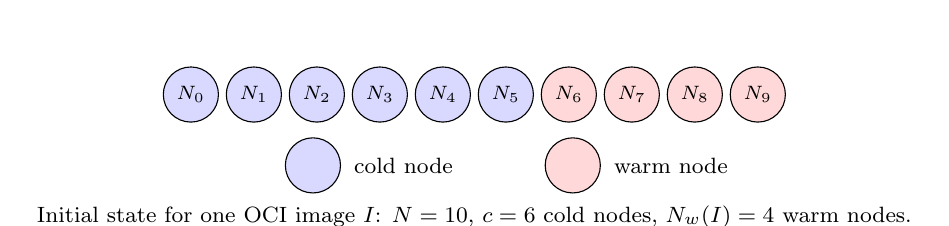
\begin{tikzpicture}[
  dot/.style={circle, draw, minimum size=7mm, inner sep=0pt, font=\scriptsize},
  cold/.style={dot, fill=blue!15},
  warm/.style={dot, fill=red!15},
  legendtext/.style={font=\footnotesize, anchor=west}
]
\node[cold] (n0) at (0,0) {$N_0$};
\node[cold] (n1) at (0.8,0) {$N_1$};
\node[cold] (n2) at (1.6,0) {$N_2$};
\node[cold] (n3) at (2.4,0) {$N_3$};
\node[cold] (n4) at (3.2,0) {$N_4$};
\node[cold] (n5) at (4.0,0) {$N_5$};
\node[warm] (n6) at (4.8,0) {$N_6$};
\node[warm] (n7) at (5.6,0) {$N_7$};
\node[warm] (n8) at (6.4,0) {$N_8$};
\node[warm] (n9) at (7.2,0) {$N_9$};

\node[cold] at (1.55,-0.9) {};
\node[legendtext] at (1.95,-0.9) {cold node};
\node[warm] at (4.85,-0.9) {};
\node[legendtext] at (5.25,-0.9) {warm node};

\node[align=center, font=\footnotesize] at (3.6,-1.55) {Initial state for one OCI image \(I\): \(N=10\), \(c=6\) cold nodes, \(N_w(I)=4\) warm nodes.};
\end{tikzpicture}
\caption{Node-dot representation of the initial cache state for one OCI image \(I\). Each dot is an eligible CI node. Light blue nodes are cold; light red nodes are warm.}
\label{fig:nodedots-initial}
\end{figure}

\subsection{Burst arrival: jobs scheduled onto cold nodes}

The burst case is introduced first because it is the clearest way to separate affected jobs from newly warmed nodes. A burst represents a group of CI job Pods created within a short scheduling window, for example a fan-out test stage. The burst assumption is not defined by a fixed number of seconds. It means that jobs in the group are scheduled before image availability changes caused by jobs in the same group can reduce exposure for later jobs in that group.

\begin{figure}[H]
\centering
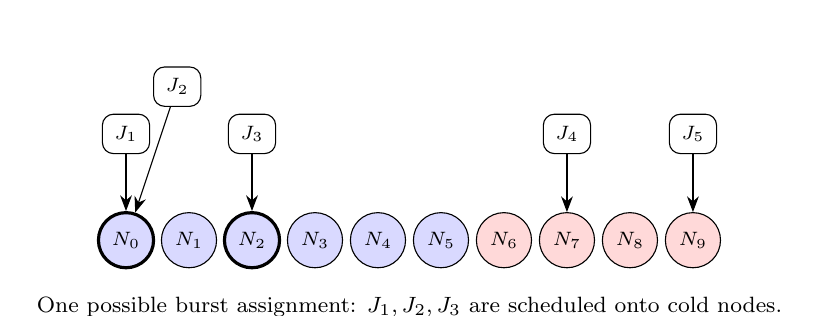
\begin{tikzpicture}[
  node distance=0.8cm,
  dot/.style={circle, draw, minimum size=7mm, inner sep=0pt, font=\scriptsize},
  cold/.style={dot, fill=blue!15},
  warm/.style={dot, fill=red!15},
  selected/.style={dot, fill=blue!15, line width=1.15pt},
  job/.style={draw, rounded corners, minimum width=6mm, minimum height=5mm, font=\scriptsize},
  arr/.style={-{Stealth[length=2mm]}, thin}
]
\node[selected] (n0) at (0,0) {$N_0$};
\node[cold]    (n1) at (0.8,0) {$N_1$};
\node[selected] (n2) at (1.6,0) {$N_2$};
\node[cold]    (n3) at (2.4,0) {$N_3$};
\node[cold]    (n4) at (3.2,0) {$N_4$};
\node[cold]    (n5) at (4.0,0) {$N_5$};
\node[warm]    (n6) at (4.8,0) {$N_6$};
\node[warm]    (n7) at (5.6,0) {$N_7$};
\node[warm]    (n8) at (6.4,0) {$N_8$};
\node[warm]    (n9) at (7.2,0) {$N_9$};

\node[job] (j1) at (0.0,1.35) {$J_1$};
\node[job] (j2) at (0.65,1.95) {$J_2$};
\node[job] (j3) at (1.6,1.35) {$J_3$};
\node[job] (j4) at (5.6,1.35) {$J_4$};
\node[job] (j5) at (7.2,1.35) {$J_5$};

\draw[arr] (j1) -- (n0);
\draw[arr] (j2) -- (n0);
\draw[arr] (j3) -- (n2);
\draw[arr] (j4) -- (n7);
\draw[arr] (j5) -- (n9);

\node[align=center, font=\footnotesize] at (3.6,-0.85) {One possible burst assignment: \(J_1,J_2,J_3\) are scheduled onto cold nodes.};
\end{tikzpicture}
\caption{Burst-arrival example for image \(I\) with \(N=10\), \(c=6\), and \(J_b=5\). Node color still shows cache state: light blue is cold and light red is warm. The arrows show one possible assignment of five jobs to nodes. This sample outcome is illustrative; the expectation below averages over all assignments under the placement baseline.}
\label{fig:nodedots-burst}
\end{figure}

If a burst starts with \(N_c(I)=c\) cold nodes, each job in the burst has probability \(c/N\) of being scheduled onto a node that is cold for \(I\). Therefore the number of affected jobs in the burst follows:
\begin{equation}
A_{\mathrm{burst}}(I)\mid N_c(I)=c
\sim
\mathrm{Binomial}\left(J_b,\frac{c}{N}\right).
\end{equation}

The expected number of affected jobs is:
\begin{equation}
\E[A_{\mathrm{burst}}(I)\mid N_c(I)=c]
=
J_b\frac{c}{N}.
\end{equation}

For the small example with \(N=10\), \(c=6\), and \(J_b=5\):
\begin{equation}
\E[A_{\mathrm{burst}}(I)\mid N_c(I)=6]
=
5\cdot\frac{6}{10}
=
3.
\end{equation}
Thus the burst is expected to expose three jobs to cold-node image-availability delay. In affected job-minutes, this is:
\begin{equation}
\E[M_{\mathrm{burst}}(I)\mid N_c(I)=c]
=
\E[A_{\mathrm{burst}}(I)\mid N_c(I)=c]\cdot\frac{p_I}{60}.
\end{equation}
With \(p_I=60\) seconds, the small burst produces an expected three affected job-minutes.

\subsection{Newly warmed nodes}

Affected jobs and newly warmed nodes are different quantities. A burst can schedule several jobs onto the same cold node before image \(I\) becomes available there. Those jobs all count as affected, but the node becomes newly warm only once.

\begin{figure}[H]
\centering
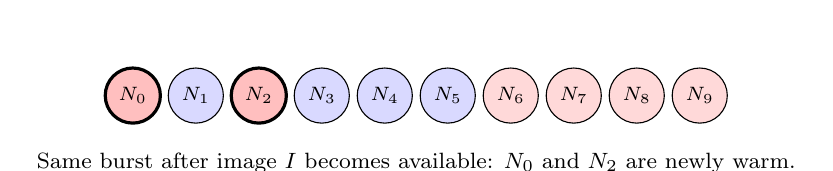
\begin{tikzpicture}[
  dot/.style={circle, draw, minimum size=7mm, inner sep=0pt, font=\scriptsize},
  cold/.style={dot, fill=blue!15},
  warm/.style={dot, fill=red!15},
  newwarm/.style={dot, fill=red!25, line width=1.15pt}
]
\node[newwarm] (n0) at (0,0) {$N_0$};
\node[cold]    (n1) at (0.8,0) {$N_1$};
\node[newwarm] (n2) at (1.6,0) {$N_2$};
\node[cold]    (n3) at (2.4,0) {$N_3$};
\node[cold]    (n4) at (3.2,0) {$N_4$};
\node[cold]    (n5) at (4.0,0) {$N_5$};
\node[warm]    (n6) at (4.8,0) {$N_6$};
\node[warm]    (n7) at (5.6,0) {$N_7$};
\node[warm]    (n8) at (6.4,0) {$N_8$};
\node[warm]    (n9) at (7.2,0) {$N_9$};
\node[align=center, font=\footnotesize] at (3.6,-0.85) {Same burst after image \(I\) becomes available: \(N_0\) and \(N_2\) are newly warm.};
\end{tikzpicture}
\caption{Cache-propagation view of the same sample outcome. Although three jobs were scheduled onto cold nodes, only two distinct nodes become newly warm because \(J_1\) and \(J_2\) were scheduled onto the same node.}
\label{fig:nodedots-cache}
\end{figure}

If a burst starts with \(c\) cold nodes for \(I\), a particular cold node is not selected by any of the \(J_b\) jobs with probability:
\begin{equation}
\left(1-\frac{1}{N}\right)^{J_b}.
\end{equation}
Therefore the expected number of newly warmed nodes is:
\begin{equation}
\E[N_{\mathrm{new}}(I)\mid N_c(I)=c]
=
c\left(1-\left(1-\frac{1}{N}\right)^{J_b}\right).
\end{equation}

For the small example:
\begin{equation}
\E[N_{\mathrm{new}}(I)\mid N_c(I)=6]
=
6\left(1-\left(1-\frac{1}{10}\right)^5\right)
\approx
2.46.
\end{equation}
The same burst is therefore expected to expose about three jobs, but to make only about 2.46 cold nodes newly warm. Several jobs can wait on the same cold node, but that node becomes newly warm only once.

The expectation is sufficient for the main examples, but the full distribution is useful for percentile bands. The cache-state distribution can be written recursively. Let \(P_n(w)\) be the probability that \(w\) nodes are warm for image \(I\) after \(n\) jobs. \(P_n(w)\) is defined for integer warm-node counts \(w\in\{0,1,\dots,N\}\). For all values outside this range, \(P_n(w)=0\). If the interval starts with \(c\) cold nodes, the initial condition is \(P_0(N-c)=1\) and \(P_0(w)=0\) for \(w
eq N-c\). Then:
\begin{equation}
P_{n+1}(w)
=
P_n(w)\frac{w}{N}
+
P_n(w-1)\frac{N-(w-1)}{N}.
\end{equation}
The first term covers jobs assigned to already warm nodes. The second term covers jobs assigned to a cold node, making one additional node warm for \(I\).

\subsection{Sequential arrival}

Sequential arrival is the opposite analytical reference case. Jobs using image \(I\) arrive one after another with enough time between them that a cold-node hit can make that node warm before the next job is scheduled. This assumption is useful for gradual traffic where cache updates can help later jobs quickly.

If the interval starts with \(N_c(I)=c\) cold nodes, then job \(j\) is affected only if it lands on a node that is still cold after the previous \(j-1\) placements. The expected number of affected jobs is:
\begin{equation}
\E[A_{\mathrm{seq}}(I)\mid N_c(I)=c]
=
c\left(1-\left(1-\frac{1}{N}\right)^J\right).
\end{equation}

This is the same occupancy expression as newly warmed nodes because, under sequential arrival, each affected job has time to make its node warm before the next job arrives. Unlike the burst case, one affected job corresponds to one newly warmed node.

For \(N=10\), \(c=6\), and \(J=5\):
\begin{equation}
\E[A_{\mathrm{seq}}(I)\mid N_c(I)=6]
=
6\left(1-\left(1-\frac{1}{10}\right)^5\right)
\approx
2.46.
\end{equation}
The sequential estimate is lower than the burst affected-job estimate of \(3.0\) because later jobs can benefit from earlier cache updates.

The affected job-minute estimate is:
\begin{equation}
\E[M_{\mathrm{seq}}(I)\mid N_c(I)=c]
=
\E[A_{\mathrm{seq}}(I)\mid N_c(I)=c]\cdot\frac{p_I}{60}.
\end{equation}

\subsection{Kubernetes interpretation}

Kubernetes makes the distinction between affected jobs and newly warmed nodes operationally important. Kubelet ensures image availability before starting containers. By default, kubelet serializes image pulls per node, while different nodes can pull in parallel. This means several Pods on one cold node may wait on the same node-local image availability process. The exact behavior depends on kubelet and runtime configuration, so it should be measured for the target cluster. The model therefore counts jobs scheduled onto cold nodes separately from nodes that become newly warm \cite{kubernetesimages}.

The model does not require every affected job to trigger an independent pull of image \(I\). It only counts that the job was scheduled onto a node where \(I\) was not yet available for its startup path.

\subsection{Affected job-minutes}

Affected job-minutes convert modeled job exposure into aggregate developer waiting exposure. For the burst and sequential reference cases, the estimates are:
\begin{align}
  \E[M_{\mathrm{burst}}(I)]
  &=
  \frac{\E[A_{\mathrm{burst}}(I)]\cdot p_I}{60}, \\
  \E[M_{\mathrm{seq}}(I)]
  &=
  \frac{\E[A_{\mathrm{seq}}(I)]\cdot p_I}{60}.
\end{align}
This metric is not wall-clock runtime. It counts aggregate waiting exposure across jobs. For burst scheduling, it assumes each job scheduled onto a cold node experiences the modeled delay \(p_I\). The observed wall-clock delay can differ because jobs may wait in parallel, share node-local image availability work, or experience additional registry and runtime contention.

For the small example with \(p_I=60\) seconds, the burst arrival estimate is:
\begin{equation}
  \frac{3\cdot 60}{60}=3
  \text{ affected job-minutes}.
\end{equation}
The sequential estimate is:
\begin{equation}
  \frac{2.46\cdot 60}{60}=2.46
  \text{ affected job-minutes}.
\end{equation}

Real CI systems often sit between the sequential and full-burst reference cases. The next section makes this rolling-concurrency case explicit.


\section{Rolling-Concurrency Extension}\label{sec:rolling-concurrency}

The previous section introduced rolling concurrency as the operational middle case between sequential arrival and full-burst arrival. This section makes that middle case explicit. A runner fleet may keep up to \(K\) jobs active, and whenever one job finishes, another queued job is scheduled. Early jobs may therefore observe a cold cache for image \(I\), while later jobs may benefit from image-availability work completed by earlier jobs.

This section does not replace the closed-form model; it explains why real CI behavior may lie between the sequential and burst reference cases.

\subsection{Availability-time model}

Let \(K\) be the maximum number of active CI job Pods:
\begin{equation}
  \#\mathrm{active\ jobs}(t) \le K.
\end{equation}
Here \(K\) is a workload-level concurrency limit, not a node count. The active jobs may be scheduled onto fewer than \(K\) nodes, and several jobs may run or wait on the same node if resources allow.

For one OCI image \(I\), the rolling model tracks the time at which \(I\) becomes available on each node. Let \(S_j\) be the scheduling time of job \(j\), \(X_j\) the node chosen for job \(j\), \(R_j\) its useful build or test runtime after image availability, and \(T_n(I)\) the time when node \(n\) has image \(I\) available for job startup.

If image \(I\) is already available on node \(X_j\) at scheduling time \(S_j\), then:
\begin{equation}
  W_j = 0.
\end{equation}

If job \(j\) is the first job using \(I\) scheduled onto a cold node \(n\), the model sets:
\begin{equation}
  T_n(I) = S_j + p_I.
\end{equation}
The job waits:
\begin{equation}
  W_j = p_I.
\end{equation}

If another job is scheduled onto the same node while image availability work is already in progress, it waits only for the remaining time:
\begin{equation}
  W_j = \max(0, T_{X_j}(I) - S_j).
\end{equation}

The job completion time is:
\begin{equation}
  F_j = S_j + W_j + R_j.
\end{equation}

The \(T_n(I)\) abstraction hides runtime-internal details such as image-pull serialization, layer reuse, and pull sharing. It represents their combined observable effect: the time at which image \(I\) becomes available on node \(n\). In the figures, a light-blue prefix at the start of a job bar means that the job is waiting because node \(X_j\) is not yet warm for image \(I\). A gray segment marks useful build or test runtime after image availability.

\subsection{Example: sequential, rolling, and full-burst arrival}

Consider \(N=2\) nodes, \(K=2\) active jobs, \(p_I=60\) seconds, and four jobs using image \(I\). Both nodes start without image \(I\). The placement sequence is:
\[
X_1=N_0,\quad X_2=N_0,\quad X_3=N_1,\quad X_4=N_1.
\]
The useful runtimes after image availability are \(R_1=60\) seconds, \(R_2=90\) seconds, \(R_3=30\) seconds, and \(R_4=30\) seconds. The same job set and placement sequence are evaluated under sequential arrival, rolling concurrency, and full-burst arrival.

For the rolling-concurrency case, jobs \(J_1\) and \(J_2\) are active at \(t=0\) and both are scheduled onto \(N_0\). The first job defines \(T_{N_0}(I)=60\), so both jobs wait 60 seconds for image \(I\). \(J_1\) finishes at \(t=120\), which frees one concurrency slot. \(J_3\) is then scheduled onto \(N_1\), defining \(T_{N_1}(I)=180\). \(J_2\) finishes at \(t=150\), so \(J_4\) is scheduled onto \(N_1\) while \(N_1\) is still unavailable. It waits only until \(T_{N_1}(I)=180\), so it waits 30 seconds.

\begin{table}[H]
\centering
\caption{Rolling-concurrency example with \(N=2\), \(K=2\), and \(p_I=60\) seconds. Waiting is measured only for image \(I\) availability; useful runtime is shown to explain when the next queued job can start.}
\label{tab:rolling-example}
\small
\begin{tabular}{lrrrrrr}
\toprule
Job & \(S_j\) & \(X_j\) & \(T_{X_j}(I)\) & \(W_j\) & \(R_j\) & \(F_j\) \\
\midrule
\(J_1\) & 0 & \(N_0\) & 60 & 60 & 60 & 120 \\
\(J_2\) & 0 & \(N_0\) & 60 & 60 & 90 & 150 \\
\(J_3\) & 120 & \(N_1\) & 180 & 60 & 30 & 210 \\
\(J_4\) & 150 & \(N_1\) & 180 & 30 & 30 & 210 \\
\bottomrule
\end{tabular}
\end{table}

The rolling-concurrency image wait is therefore:
\begin{equation}
  D_{\mathrm{roll}}
  =
  60 + 60 + 60 + 30
  =
  210\text{ seconds}
  =
  3.5\text{ affected job-minutes}.
\end{equation}

\begin{figure}[H]

\begin{adjustbox}{max width=0.96\textwidth}
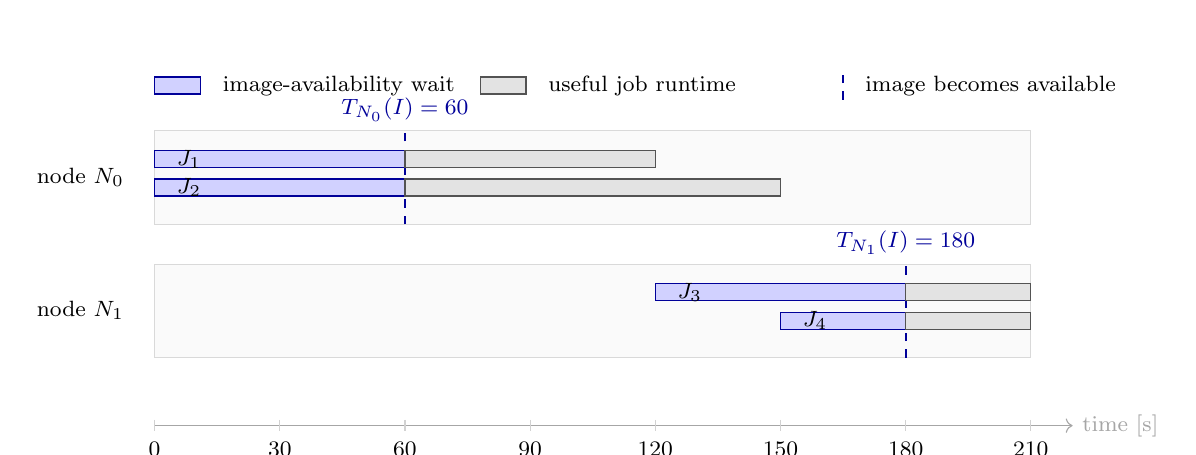
\begin{tikzpicture}[
  x=0.053cm,
  y=0.72cm,
  lane/.style={draw=gray!30, fill=gray!4},
  coldwait/.style={fill=blue!18, draw=blue!60!black},
  runtime/.style={fill=gray!22, draw=gray!65!black},
  avail/.style={draw=blue!60!black, dashed, thick},
  label/.style={font=\footnotesize},
  joblabel/.style={font=\footnotesize, anchor=west},
  axislabel/.style={font=\footnotesize}
]
% axis
\draw[->, gray!70] (0,0) -- (220,0) node[right, axislabel] {time [s]};
\foreach \x in {0,30,60,90,120,150,180,210} {
  \draw[gray!35] (\x,0.10) -- (\x,-0.10);
  \node[axislabel, anchor=north] at (\x,-0.12) {\x};
}

% node lanes
\draw[lane] (0,3.55) rectangle (210,5.20);
\draw[lane] (0,1.20) rectangle (210,2.85);
\node[label, anchor=east] at (-5,4.38) {node $N_0$};
\node[label, anchor=east] at (-5,2.03) {node $N_1$};

% availability markers
\draw[avail] (60,3.55) -- (60,5.20);
\node[axislabel, anchor=south, blue!60!black] at (60,5.20) {$T_{N_0}(I)=60$};
\draw[avail] (180,1.20) -- (180,2.85);
\node[axislabel, anchor=south, blue!60!black] at (180,2.85) {$T_{N_1}(I)=180$};

% N0 jobs
\draw[coldwait] (0,4.55) rectangle (60,4.85);
\draw[runtime] (60,4.55) rectangle (120,4.85);
\node[joblabel] at (3,4.70) {$J_1$};
\draw[coldwait] (0,4.05) rectangle (60,4.35);
\draw[runtime] (60,4.05) rectangle (150,4.35);
\node[joblabel] at (3,4.20) {$J_2$};

% N1 jobs
\draw[coldwait] (120,2.20) rectangle (180,2.50);
\draw[runtime] (180,2.20) rectangle (210,2.50);
\node[joblabel] at (123,2.35) {$J_3$};
\draw[coldwait] (150,1.70) rectangle (180,2.00);
\draw[runtime] (180,1.70) rectangle (210,2.00);
\node[joblabel] at (153,1.85) {$J_4$};

% legend
\draw[coldwait] (0,5.85) rectangle (11,6.15);
\node[axislabel, anchor=west] at (14,6.00) {image-availability wait};
\draw[runtime] (78,5.85) rectangle (89,6.15);
\node[axislabel, anchor=west] at (92,6.00) {useful job runtime};
\draw[avail] (165,5.75) -- (165,6.25);
\node[axislabel, anchor=west] at (168,6.00) {image becomes available};
\end{tikzpicture}
\end{adjustbox}
\caption{Rolling-concurrency example. Jobs \(J_1\) and \(J_2\) both wait a full \(p_I=60\) seconds on \(N_0\). Job \(J_4\) starts while image \(I\) is still unavailable on \(N_1\) and waits only the remaining 30 seconds until \(T_{N_1}(I)\).}
\label{fig:rolling-node-timeline}
\end{figure}

In the sequential special case \(K=1\), only the first job on each node waits: \(J_1\) waits 60 seconds on \(N_0\), \(J_2\) waits 0, \(J_3\) waits 60 seconds on \(N_1\), and \(J_4\) waits 0. Thus:
\begin{equation}
  D_{\mathrm{seq}} = 120\text{ seconds} = 2.0\text{ affected job-minutes}.
\end{equation}
In the full-burst special case, all four jobs are scheduled before either node becomes warm. Each job waits 60 seconds:
\begin{equation}
  D_{\mathrm{burst}} = 240\text{ seconds} = 4.0\text{ affected job-minutes}.
\end{equation}
The rolling-concurrency example lies between those analytical reference cases:
\begin{equation}
  D_{\mathrm{seq}} = 2.0
  \le
  D_{\mathrm{roll}} = 3.5
  \le
  D_{\mathrm{burst}} = 4.0.
\end{equation}

\begin{figure}[H]
\centering
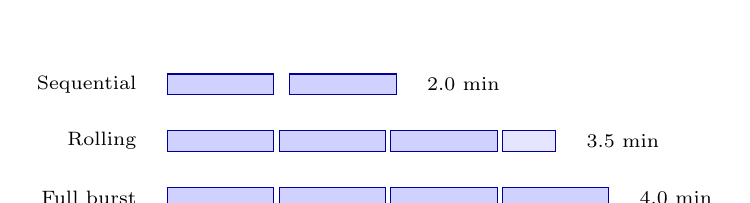
\begin{tikzpicture}[
  x=1.35cm,
  y=0.72cm,
  full/.style={fill=blue!18, draw=blue!60!black},
  partial/.style={fill=blue!10, draw=blue!60!black},
  label/.style={font=\scriptsize},
  rowlabel/.style={font=\scriptsize, anchor=east}
]
\node[rowlabel] at (-0.2,3) {Sequential};
\draw[full] (0,2.82) rectangle (1,3.18);
\draw[full] (1.15,2.82) rectangle (2.15,3.18);
\node[label, anchor=west] at (2.35,3) {2.0 min};
\node[rowlabel] at (-0.2,2) {Rolling};
\draw[full] (0,1.82) rectangle (1,2.18);
\draw[full] (1.05,1.82) rectangle (2.05,2.18);
\draw[full] (2.10,1.82) rectangle (3.10,2.18);
\draw[partial] (3.15,1.82) rectangle (3.65,2.18);
\node[label, anchor=west] at (3.85,2) {3.5 min};
\node[rowlabel] at (-0.2,1) {Full burst};
\draw[full] (0,0.82) rectangle (1,1.18);
\draw[full] (1.05,0.82) rectangle (2.05,1.18);
\draw[full] (2.10,0.82) rectangle (3.10,1.18);
\draw[full] (3.15,0.82) rectangle (4.15,1.18);
\node[label, anchor=west] at (4.35,1) {4.0 min};
\end{tikzpicture}
\caption{Comparison of the same deterministic example under all three modes. The rolling case is a time-aware operational case between the sequential and full-burst analytical references. Each full block represents one \(p_I=60\) second image wait; the half block represents a 30 second remaining wait.}
\label{fig:rolling-boundary-check}
\end{figure}


\subsection{Developer-time weighting in rolling concurrency}

Developer-weighted rolling waiting for a realized scheduling trace can be written as:
\begin{equation}
  D_{\mathrm{roll}}
  =
  \sum_j
  \int_{S_j}^{S_j+W_j} f(t)\,dt.
\end{equation}
The integral counts the overlap between image-wait intervals and the developer-time weight \(f(t)\). Waiting outside developer-relevant time may still warm nodes, but it contributes little or nothing to developer-facing cold-node exposure. Under stochastic placement or runtime assumptions, the model estimates \(\E[D_{\mathrm{roll}}]\), typically by event simulation.

For the numerical scenario used later, wall-clock time \(t\) is measured within one modeled day and the developer-time weight is:
\begin{equation}
 f(t)=
 \begin{cases}
 0, & 00{:}00 \le t < 07{:}00,\\
 0.3, & 07{:}00 \le t < 09{:}00,\\
 1, & 09{:}00 \le t < 17{:}00,\\
 0.3, & 17{:}00 \le t < 20{:}00,\\
 0, & 20{:}00 \le t < 24{:}00.
 \end{cases}
\end{equation}
The values are scenario assumptions, not a claim that every developer works exactly these hours. They make the model explicit about which waiting intervals should count strongly as developer-facing CI exposure.

\begin{figure}[H]
\centering
\begin{adjustbox}{max width=0.86\linewidth}
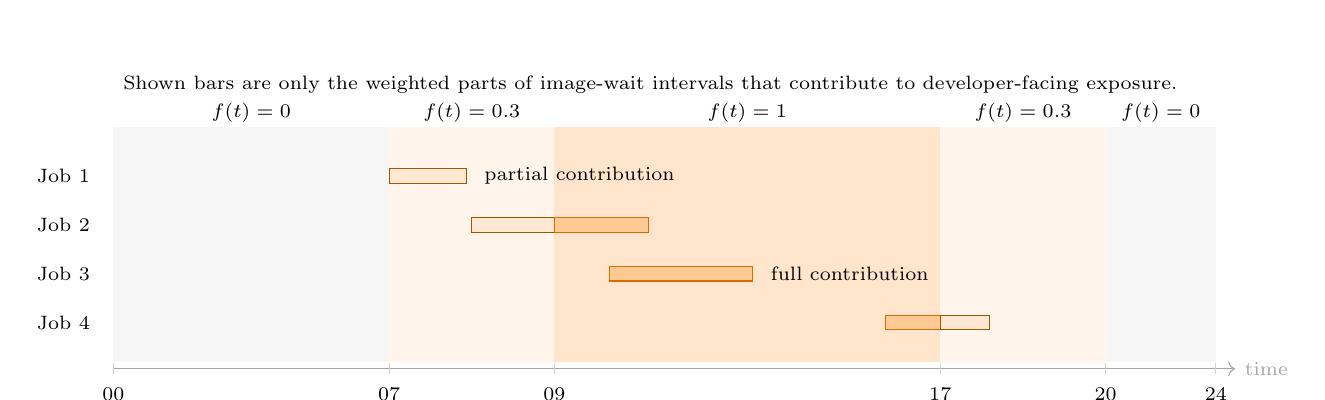
\begin{tikzpicture}[
  x=0.70cm,
  y=0.62cm,
  countedLow/.style={fill=orange!18, draw=orange!65!black},
  countedHigh/.style={fill=orange!42, draw=orange!85!black},
  axislabel/.style={font=\scriptsize},
  joblabel/.style={font=\scriptsize, anchor=east}
]
\path[fill=gray!7] (0,0.6) rectangle (5,5.4);
\path[fill=orange!8] (5,0.6) rectangle (8,5.4);
\path[fill=orange!20] (8,0.6) rectangle (15,5.4);
\path[fill=orange!8] (15,0.6) rectangle (18,5.4);
\path[fill=gray!7] (18,0.6) rectangle (20,5.4);

\node[axislabel] at (2.5,5.70) {$f(t)=0$};
\node[axislabel] at (6.5,5.70) {$f(t)=0.3$};
\node[axislabel] at (11.5,5.70) {$f(t)=1$};
\node[axislabel] at (16.5,5.70) {$f(t)=0.3$};
\node[axislabel] at (19.0,5.70) {$f(t)=0$};

\draw[->, gray!70] (0,0.45) -- (20.35,0.45) node[right, axislabel] {time};
\foreach \x/\lab in {0/00,5/07,8/09,15/17,18/20,20/24} {
  \draw[gray!35] (\x,0.56) -- (\x,0.34);
  \node[axislabel, anchor=north] at (\x,0.25) {\lab};
}

\node[joblabel] at (-0.25,4.4) {Job 1};
\draw[countedLow] (5.0,4.25) rectangle (6.4,4.55);
\node[axislabel, anchor=west] at (6.55,4.40) {partial contribution};

\node[joblabel] at (-0.25,3.4) {Job 2};
\draw[countedLow] (6.5,3.25) rectangle (8.0,3.55);
\draw[countedHigh] (8.0,3.25) rectangle (9.7,3.55);

\node[joblabel] at (-0.25,2.4) {Job 3};
\draw[countedHigh] (9.0,2.25) rectangle (11.6,2.55);
\node[axislabel, anchor=west] at (11.75,2.40) {full contribution};

\node[joblabel] at (-0.25,1.4) {Job 4};
\draw[countedHigh] (14.0,1.25) rectangle (15.0,1.55);
\draw[countedLow] (15.0,1.25) rectangle (15.9,1.55);

\node[axislabel, anchor=west] at (0,6.28) {Shown bars are only the weighted parts of image-wait intervals that contribute to developer-facing exposure.};
\end{tikzpicture}
\end{adjustbox}
\caption{Developer-time weighting for image-wait intervals. Only the counted weighted overlap is shown: waiting during \(f(t)=0\) is omitted, shoulder-period waiting contributes partially, and waiting during the main developer feedback window contributes fully.}
\label{fig:developer-weighted-wait}
\end{figure}

For a closed-form model, the paper keeps sequential and full-burst arrival as analytical bounds. For a node \(n\) where image \(I\) is initially unavailable and \(M_n>0\) jobs using \(I\) are scheduled onto it before \(T_n(I)\):
\begin{equation}
  p_I
  \le
  \sum_{j:X_j=n} W_j
  \le
  p_I M_n.
\end{equation}
The lower bound corresponds to the sequential-style case where only the first job waits a full \(p_I\). The upper bound corresponds to the full-burst case where all \(M_n\) jobs are scheduled before image availability can make progress. Rolling concurrency lies between these bounds because jobs can be scheduled before \(T_n(I)\) and therefore wait only the remaining time.

The operational rolling model is best evaluated by event simulation: keep up to \(K\) jobs active, schedule a new job whenever one finishes, track \(T_n(I)\) per node, and count the waiting time seen by jobs scheduled before image \(I\) is available on their assigned node.



\section{Single-Image Node Rotation Scenario}\label{sec:primary-scenario}

This numerical scenario evaluates a dedicated Kubernetes node pool for CI jobs, such as jobs executed by the GitLab Kubernetes executor. The scenario places node rotation before the main developer feedback window. This timing represents an off-hours maintenance event, but the same model also applies to rotations caused by security updates, upgrades, or infrastructure replacement at other times of day.

Node replacement creates healthy, schedulable nodes, but it does not retain the node-local image cache of the replaced nodes. Immediately after the 00:00 rotation, the modeled OCI image \(I\) is therefore cold on every node in the CI pool:
\[
N_w(I,00{:}00)=0,\qquad N_c(I,00{:}00)=N.
\]

\begin{table}[H]
\centering
\caption{Parameters for the representative CI node-pool rotation scenario. Image-specific job counts refer only to jobs using the modeled OCI image digest.}
\label{tab:main-scenario-parameters}
\small
\begin{tabular}{lr}
\toprule
Parameter & Value \\
\midrule
Eligible CI nodes \(N\) & 100 \\
Total CI/CD jobs per day & 25,000 \\
Image \(I\) share of CI traffic & 2\% \\
Jobs using image \(I\) before developer window & 70.7 \\
Rotation time & 00:00 \\
Developer feedback window & 09:00--17:00 \\
Cold-node image-availability time \(p_I\) & 60 seconds \\
Jobs using image \(I\) in developer window & 500 \\
Rolling-concurrency limit \(K\) & 100 active jobs \\
\bottomrule
\end{tabular}
\end{table}

These values are illustrative scenario parameters. In a production study, the job-volume distribution, image-specific job counts, and cold-node image-availability time should be measured. In this example, image \(I\) is assumed to account for 2\% of total CI traffic. Applied to the 00:00--09:00 traffic profile, that yields 70.7 jobs using image \(I\) before the developer feedback window.

\subsection{Daily traffic and developer-time weighting}

The daily average is:
\begin{equation}
  \frac{25{,}000}{24\cdot 60}=17.36 \text{ jobs/minute}.
\end{equation}
CI traffic usually follows work patterns, so a uniform distribution would hide the difference between background activity and developer-facing feedback time. The scenario therefore uses nonzero night traffic, a morning ramp-up, a developer-day peak, an evening tail, and low background activity at night.

The scenario uses the developer-time weight \(f(t)\) defined in Section~\ref{sec:rolling-concurrency}: \(f(t)=1\) during the main developer feedback window from 09:00 to 17:00, \(f(t)=0.3\) during the shoulder periods 07:00--09:00 and 17:00--20:00, and \(f(t)=0\) at night. Total CI volume describes when work enters the CI system; jobs using image \(I\) determine cache warming; \(f(t)\) determines how strongly affected job-minutes are interpreted as developer-facing cold-node exposure.

\begin{figure}[H]
\centering
\begin{adjustbox}{max width=0.94\linewidth}
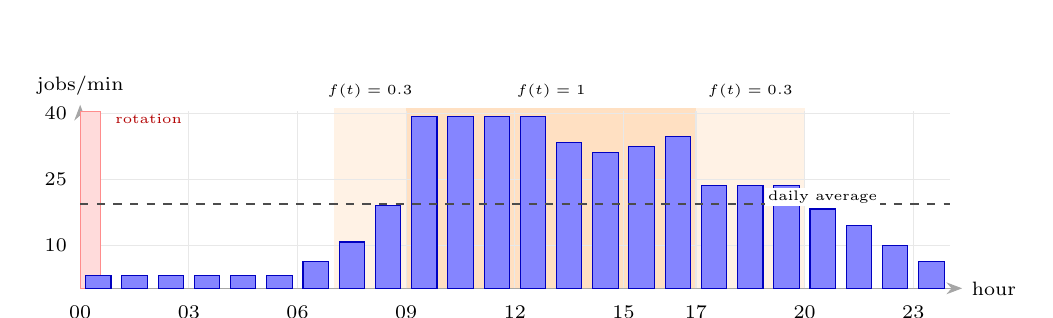
\begin{tikzpicture}[
  x=0.46cm,
  y=0.42cm,
  label/.style={font=\scriptsize},
  tinylabel/.style={font=\tiny},
  loadbar/.style={fill=blue!48, draw=blue!75!black},
  shoulder/.style={fill=orange!10, draw=none},
  developer/.style={fill=orange!24, draw=none},
  axis/.style={draw=gray!70, -{Stealth[length=2mm]}},
  guide/.style={draw=gray!18}
]
\path[shoulder] (7,0.7) rectangle (9,6.15);
\path[developer] (9,0.7) rectangle (17,6.15);
\path[shoulder] (17,0.7) rectangle (20,6.15);
\draw[axis] (0,0.7) -- (24.35,0.7) node[anchor=west,label] {hour};
\draw[axis] (0,0.7) -- (0,6.25) node[anchor=south,label] {jobs/min};
\foreach \x/\lab in {0/00,3/03,6/06,9/09,12/12,15/15,17/17,20/20,23/23} {
  \draw[guide] (\x,0.7) -- (\x,6.05);
  \node[label, anchor=north] at (\x,0.45) {\lab};
}
\foreach \y/\lab in {2/10,4/25,6/40} {
  \draw[guide] (0,\y) -- (24,\y);
  \node[label, anchor=east] at (-0.10,\y) {\lab};
}
\path[fill=red!14, draw=red!45] (0,0.7) rectangle (0.55,6.05);
\node[tinylabel, anchor=west, red!70!black] at (0.70,5.82) {rotation};
\foreach \x/\h in {
0/1.1,1/1.1,2/1.1,3/1.1,4/1.1,5/1.1,
6/1.5,7/2.1,8/3.2,9/5.9,10/5.9,11/5.9,12/5.9,
13/5.1,14/4.8,15/5.0,16/5.3,17/3.8,18/3.8,19/3.8,
20/3.1,21/2.6,22/2.0,23/1.5} {
  \draw[loadbar] (\x+0.15,0.7) rectangle (\x+0.85,\h);
}
\draw[dashed, thick, black!70] (0,3.25) -- (24,3.25);
\node[tinylabel, anchor=west, fill=white, inner sep=1pt] at (18.9,3.45) {daily average};
\node[tinylabel, anchor=south] at (8,6.16) {\(f(t)=0.3\)};
\node[tinylabel, anchor=south] at (13,6.16) {\(f(t)=1\)};
\node[tinylabel, anchor=south] at (18.5,6.16) {\(f(t)=0.3\)};
\end{tikzpicture}
\end{adjustbox}
\caption{Compact scenario timeline for the numerical model. Bars show total CI job volume by hour. Background bands define the developer-time weight \(f(t)\): no weighting outside developer-relevant periods, partial weighting during shoulder periods, and full weighting during the main developer feedback window.}
\label{fig:dailyoverlap}
\end{figure}


After the 00:00 rotation, image \(I\) is cold on all 100 CI nodes. Between 00:00 and 09:00, about 70.7 CI jobs use image \(I\). Under the newly warmed-node expectation, this background traffic warms only about 50.9 nodes by the start of the developer feedback window.

\begin{table}[H]
\centering
\caption{Cache-state progression after the CI node-pool rotation. The table tracks jobs using image \(I\), not all CI jobs.}
\label{tab:nightcache}
\small
\begin{adjustbox}{max width=\linewidth}
\begin{tabular}{lrrr}
\toprule
Time & Target-image jobs since 00:00 & Expected warm nodes & Expected cold nodes \\
\midrule
00:00 & 0.0 & 0.0 & 100.0 \\
01:00 & 4.3 & 4.2 & 95.8 \\
02:00 & 8.6 & 8.3 & 91.7 \\
03:00 & 12.9 & 12.2 & 87.8 \\
04:00 & 17.2 & 15.9 & 84.1 \\
05:00 & 21.6 & 19.5 & 80.5 \\
06:00 & 25.9 & 22.9 & 77.1 \\
07:00 & 37.9 & 31.7 & 68.3 \\
08:00 & 50.0 & 39.5 & 60.5 \\
09:00 & 70.7 & 50.9 & 49.1 \\
\bottomrule
\end{tabular}

\end{adjustbox}
\end{table}

\begin{figure}[H]
\centering
\begin{tikzpicture}
\begin{axis}[
  width=0.90\linewidth,
  height=5.6cm,
  xlabel={Clock time},
  ylabel={Expected warm nodes},
  xmin=0,xmax=9,
  ymin=0,ymax=105,
  xtick={0,2,4,6,8,9},
  xticklabels={00:00,02:00,04:00,06:00,08:00,09:00},
  grid=major,
  grid style={draw=gray!15},
]
\addplot+[very thick,mark=*,orange!85!black] table[x=time,y=normal_warm_nodes,col sep=comma] {generated/night_cache_progress_dense.csv};
\addplot+[dashed,thick,green!50!black,mark=none] coordinates {(0,100) (9,100)};
\addplot+[dashed,thick,black,mark=none] coordinates {(9,0) (9,105)};
\node[anchor=west,font=\scriptsize] at (axis cs:4.2,38) {warming from normal CI traffic};
\node[anchor=west,font=\scriptsize,green!45!black] at (axis cs:0.25,93) {all nodes warm};
\node[anchor=east,font=\scriptsize] at (axis cs:8.86,13) {developer feedback window};
\end{axis}
\end{tikzpicture}
\caption{Expected cache-warming progress for image \(I\) between the 00:00 rotation and the 09:00 developer feedback window. Normal background traffic warms only part of the CI node pool before the high-weight developer feedback window begins.}
\label{fig:nightcacheprogress}
\end{figure}


\subsection{Rolling-concurrency impact at 09:00}

At 09:00, \(f(t)=1\) in the scenario, so affected job-minutes during this period are interpreted as full developer-facing cold-node exposure. About 49.1 nodes remain cold for image \(I\). If the next 500 CI jobs using image \(I\) run during developer time, the remaining cold state can still delay feedback.

To connect the scenario to GitLab Kubernetes executor behavior, this section uses a coarse rolling-concurrency approximation with \(K=100\) active jobs. The 500 developer feedback window jobs are processed as five active sets of 100 jobs. This is not a full event simulation; it assumes that image-availability work triggered by one active set is visible before the next active set is scheduled. The production replay method in Section~\ref{sec:real-cluster-benchmark-methodology} replaces this approximation with observed scheduling times \(S_j\), node placements \(X_j\), and image availability times \(T_n(I)\).

For active set \(r\), let \(c_r\) be the expected number of cold nodes for image \(I\) at the start of that set. The expected affected jobs and newly warmed nodes are:
\begin{align}
  \E[A_r(I)] &= K\frac{c_r}{N},\\
  \E[N_{\mathrm{new},r}(I)] &= c_r\left(1-\left(1-\frac{1}{N}\right)^K\right),\\
  c_{r+1} &= c_r - \E[N_{\mathrm{new},r}(I)].
\end{align}

\begin{table}[H]
\centering
\caption{Rolling-concurrency approximation at the 09:00 developer feedback window for one image \(I\). The table shows how cold-node exposure and cache warming evolve across five active sets of 100 jobs.}
\label{tab:morningrolling}
\small
\begin{adjustbox}{max width=\linewidth}
\begin{tabular}{rrrrr}
\toprule
Active set & Cold nodes at start & Expected affected jobs & Newly warmed nodes & Cold nodes after \\
\midrule
1 & 49.10 & 49.10 & 31.13 & 17.97 \\
2 & 17.97 & 17.97 & 11.39 & 6.58 \\
3 & 6.58 & 6.58 & 4.17 & 2.41 \\
4 & 2.41 & 2.41 & 1.53 & 0.88 \\
5 & 0.88 & 0.88 & 0.56 & 0.32 \\
\midrule
Total & -- & 76.94 & -- & -- \\
\bottomrule
\end{tabular}

\end{adjustbox}
\end{table}

With \(p_I=60\) seconds, this approximation gives about \(76.94\) affected job-minutes for image \(I\). For comparison, a sequential reference with the same 500 jobs gives about \(48.78\) affected job-minutes, while a full 500-job burst at 09:00 would give \(245.50\) affected job-minutes. The rolling-concurrency scenario is therefore the operational middle case: jobs are not perfectly sequential, but cache updates can still help later jobs after earlier active sets have made nodes warm.

The per-developer average is only a normalization and is not part of the stochastic model. If \(76.94\) developer-facing affected job-minutes are distributed across 100 developers, that is \(0.77\) minutes per developer on average, but real waiting time is concentrated among developers whose jobs use image \(I\) during the cold event.

\section{Portfolio Extension for the Numerical Scenario}\label{sec:multi-image}

The single-image scenario explains one OCI image \(I\). A real CI system usually uses many OCI images: language runtimes, build images, test images, Docker build images, deployment tooling, and project-specific images. This section applies the same numerical node-rotation scenario to 30 illustrative CI images.

Let \(\mathcal{I}=\{I_1,I_2,\dots,I_m\}\) be the set of modeled CI images. For each image \(I\in\mathcal{I}\), let \(J_{I,\mathrm{pre}}\) be the number of jobs using \(I\) between the 00:00 rotation and the 09:00 developer feedback window, \(J_{I,\mathrm{dev}}\) the number of developer feedback window jobs using \(I\), \(N_c(I)\) the expected cold-node count for \(I\) at 09:00 after pre-window background warming, and \(p_I\) the cold-node image-availability time for \(I\).

For a simple portfolio prioritization score, the paper uses the cold-node fraction at developer feedback window start, the developer feedback window job count, and the image-availability time. This burst-style score is not a full rolling replay; it is a compact ranking signal that can later be replaced by the GitLab executor replay method. The estimated waiting contribution of image \(I\) is:
\begin{equation}
  D_I
  =
  \frac{J_{I,\mathrm{dev}}(N_c(I)/N)p_I}{60}.
\end{equation}
The portfolio estimate is:
\begin{equation}
  D_{\mathrm{portfolio}}
  =
  \sum_{I\in\mathcal{I}} D_I.
\end{equation}

\begin{table}[H]
\centering
\caption{Portfolio application for the midnight-rotation scenario. The table ranks CI images by estimated developer waiting contribution \(D_I\). The values are illustrative inputs for a 25,000-job day on a 100-node CI pool; production inputs should be measured from CI history, Kubernetes workload data, registry data, or monitoring data.}
\label{tab:multiimage}
\scriptsize
\begin{adjustbox}{max width=\linewidth}
\begin{tabular}{lrrrrr}
\toprule
Image & \(J_{i,\mathrm{pre}}\) & \(J_{i,\mathrm{dev}}\) & Cold nodes at 09:00 & \(p_i\) [s] & \(D_i\) [min] \\
\midrule
img-09 & 70.6 & 95 & 49.2 & 210 & 163.53 \\
img-03 & 148.1 & 180 & 22.6 & 180 & 121.94 \\
img-07 & 95.7 & 115 & 38.2 & 150 & 109.92 \\
img-15 & 44.4 & 52 & 64.0 & 170 & 94.28 \\
img-05 & 113.9 & 140 & 31.8 & 120 & 89.14 \\
img-12 & 54.7 & 70 & 57.7 & 130 & 87.55 \\
img-22 & 26.2 & 26 & 76.9 & 220 & 73.27 \\
img-11 & 59.2 & 78 & 55.1 & 95 & 68.10 \\
\bottomrule
\end{tabular}

\end{adjustbox}
\end{table}

Across the 30-image portfolio, the model estimates \(1{,}512.28\) affected job-minutes, or about \(25.20\) affected job-hours, during the developer window that follows one rotation event. The top five images account for \(578.81\) affected job-minutes, while the top ten account for \(923.02\) affected job-minutes. In this scenario, image prewarming is therefore a prioritization problem: warming the highest-contribution images first removes the largest share of developer-facing waiting exposure.

\begin{figure}[H]
\centering
\begin{tikzpicture}
\begin{axis}[
  width=0.90\linewidth,
  height=5.6cm,
  xlabel={Images included in priority order},
  ylabel={Cumulative affected job-minutes},
  xmin=1,xmax=30,
  ymin=0,
  xtick={1,5,10,15,20,25,30},
  grid=major,
  grid style={draw=gray!15},
]
\addplot[name path=portfolio, draw=none] table[x=top_k,y=cumulative_feedback_minutes,col sep=comma] {generated/multi_image_cumulative.csv};
\addplot[name path=baseline, draw=none] coordinates {(1,0) (30,0)};
\addplot[blue!12] fill between[of=portfolio and baseline];
\addplot+[very thick,mark=*,blue!80!black] table[x=top_k,y=cumulative_feedback_minutes,col sep=comma] {generated/multi_image_cumulative.csv};
\draw[dashed,gray!70] (axis cs:5,0) -- (axis cs:5,1550);
\draw[dashed,gray!70] (axis cs:10,0) -- (axis cs:10,1550);
\node[anchor=west,font=\scriptsize] at (axis cs:5.3,210) {top 5};
\node[anchor=west,font=\scriptsize] at (axis cs:10.3,360) {top 10};
\end{axis}
\end{tikzpicture}
\caption{Cumulative affected job-minutes across the 30-image portfolio in the numerical scenario. Images are ordered by modeled contribution \(D_I\); the steep early slope shows where prewarming has the largest expected effect.}
\label{fig:multiimagecumulative}
\end{figure}

The portfolio result changes the interpretation of the single-image example. A single image may contribute about one hour of affected job-minutes, but a realistic image portfolio can accumulate more than 25 affected job-hours in the same developer window after one rotation event. This is not a steady daily loss unless the CI node pool is rotated every day. The model therefore supports both image-level analysis and portfolio-level prioritization.

\section{Kubernetes Scheduler Notes}\label{sec:scheduler-notes}

The core model counts runtime cold-node exposure. It does not depend on Kubernetes making uniform scheduling decisions in production. Real Kubernetes scheduling is score-based: the scheduler filters feasible nodes and then scores them with configured plugins. The default scheduler includes \texttt{ImageLocality}, which favors nodes already having the Pod's images, as well as resource-related plugins such as \texttt{NodeResourcesFit} and \texttt{NodeResourcesBalancedAllocation} \cite{schedulerconfig}. \texttt{ImageLocality} is a score, not a guarantee; resource scoring, topology spread, affinity, taints, and tie-breaking can override or dilute the effect.

The model uses runtime image availability state:
\[
N_w^{\mathrm{runtime}}(I)=\text{nodes where image \(I\) is locally usable for startup}.
\]
The scheduler can only score image locality from Kubernetes-visible state:
\[
N_w^{\mathrm{visible}}(I)=\text{nodes where image \(I\) is visible through node status}.
\]
These two quantities should not be treated as identical. Kubelet reports images through node status, and \texttt{nodeStatusMaxImages} caps the number of images reported in \texttt{Node.status.images}. The documented default is 50, while \texttt{-1} removes the cap \cite{kubeletconfig}. If a prewarmed image is locally present but not reported in node status, it can still reduce runtime startup delay, but \texttt{ImageLocality} may not help the scheduler choose that node.

The uniform placement assumption in Section~\ref{sec:core-model} is therefore a reference baseline, not a scheduler prediction. A production study can replace that baseline with observed placement data, measured cold-node hit rates, or a scheduler-aware simulation. The exposure metric remains the same: jobs are counted when they are scheduled onto nodes where image \(I\) is not yet available for their startup path.

\section{Prewarming Implementation and Image Discovery}

A common low-complexity prewarming baseline is a DaemonSet. Kubernetes describes a DaemonSet as ensuring that all or some nodes run a copy of a Pod, with Pods added as nodes are added \cite{kubernetesdaemonset}. Kubernetes Image Puller follows this pattern to make selected images available on each node \cite{kubernetesimagepuller}. Another operator-style project is kube-fledged, which manages image caches through declared image-cache resources \cite{kubefledged}. These tools are useful operational reference points, but this paper does not treat any one implementation as normative.

This paper uses the Drop Image Caching Operator only as a reference implementation of the automated prewarming workflow, not as the only possible solution. In contrast to a DaemonSet-based prewarmer, Drop schedules individual prewarming Pods onto selected nodes. The design goal is to make node targeting, pacing, and retry behavior explicit, while avoiding a single rigid Pod template and reducing the chance of synchronized registry pressure when many nodes would otherwise pull the same image at once \cite{drop,dropdiscovery}. The model does not require Drop; Drop is one implementation that makes the discovery and prewarming workflow operational.

The discovery problem itself is tool-neutral. The model only requires a ranked list of CI images and an estimate of how often each image is used over a relevant time window. In many production clusters, the necessary evidence is already present in monitoring systems such as Prometheus or Grafana Mimir \cite{prometheusoverview,mimiroverview}. One practical approach is to use any image-labeled container metric as an observation source and aggregate the returned series by image. In that case, the metric is only a carrier for image labels and counts; the semantic goal is not to analyze memory, CPU, or another resource, but to estimate how often each image appears in the CI workload.

The concrete Drop documentation example uses:
\begin{center}
\texttt{count(container\_memory\_working\_set\_bytes\{container!="", container!="POD", namespace="build-stuff"\}) by (image)}
\end{center}
as a practical image-count aggregation over running containers. In GitLab Kubernetes executor environments, discovery can usually be scoped by namespace and runner Pod name patterns such as \texttt{runner-.*} \cite{dropdiscovery}.

When a lookback window is used, the discovery controller does not rank images from a single instant. Instead, it queries a time range and aggregates the returned values per image over that window. Images that appear more often over the window receive larger discovery scores and are therefore more likely to be selected for prewarming. Figure~\ref{fig:usage-window-aggregation} illustrates the simplest count-based table-to-ranking step. The score is a discovery ranking signal, not a direct estimate of developer waiting contribution \(D_I\). In Drop, the resulting \texttt{\{image, score\}} pairs are written by \texttt{DiscoveryPolicy} and consumed by \texttt{CachedImageSet}, which materializes the selected images as prewarming work on the cluster \cite{dropdiscovery}. The same logic could be implemented by another controller or pipeline.


\subsection{Usage-based discovery strategies}

A practical discovery controller should start with strategies that can be computed from historical CI workload observations alone. The paper therefore treats image size and registry metadata as optional future enrichments, not as requirements for the first discovery step. The core inputs are image observations over time and, for burst-aware ranking, the number of active or starting jobs that require the same image.

Let
\begin{equation}
S_I=\sum_{\tau\in W}\mathrm{count}_I(\tau)
\end{equation}
be the total observed usage of image \(I\) over a historical window \(W\). The simplest strategy ranks images by \(S_I\). This is robust and easy to implement, but it does not distinguish developer-facing usage from background activity or concentrated batches.

A developer-time weighted strategy uses the same \(f(t)\) function as the exposure model:
\begin{equation}
\mathrm{score}_{\mathrm{dev}}(I)
=
\sum_{\tau\in W} f(\tau)\,\mathrm{count}_I(\tau).
\end{equation}
This favors images that are observed during developer-relevant periods and de-emphasizes images that are used mostly outside the developer feedback window.

A recent-window strategy ranks images by observations in the latest interval before the policy is evaluated:
\begin{equation}
\mathrm{score}_{\mathrm{recent}}(I)
=
\sum_{\tau\in(t-L,t]}\mathrm{count}_I(\tau).
\end{equation}
This adapts quickly when image usage changes, but it may overreact to short-lived spikes.

High-volume CI bursts can matter even when \(f(t)=0\), because they can concentrate image pulls and occupy runner capacity. The relevant historical signal is same-image concurrency rather than developer-time weighting. Let
\begin{equation}
C_I(\tau)=\text{active or starting CI jobs at time \(\tau\) that require image \(I\)}.
\end{equation}
A peak-concurrency score is then:
\begin{equation}
\mathrm{score}_{\mathrm{conc}}(I)=\max_{\tau\in W} C_I(\tau).
\end{equation}
This ranks images that appear in concentrated fan-out stages or scheduled batches, even if those batches occur outside the developer feedback window.

A conservative hybrid strategy combines total usage and peak concurrency after normalizing both scores across candidate images:
\begin{equation}
\mathrm{score}_{\mathrm{hybrid}}(I)
=
\alpha\,\mathrm{norm}(S_I)
+
(1-\alpha)\,\mathrm{norm}(\mathrm{score}_{\mathrm{conc}}(I)),
\qquad 0\le\alpha\le 1.
\end{equation}
This gives a controller both popularity and burst-awareness without requiring image-size metadata or pull-time estimates. Table~\ref{tab:discovery-strategies} summarizes these usage-based strategies.

\begin{table}[H]
\centering
\caption{Usage-based discovery strategies that can be computed from historical CI image observations. These strategies do not require image-size metadata.}
\label{tab:discovery-strategies}
\scriptsize
\begin{adjustbox}{max width=\linewidth}
\begin{tabular}{p{0.22\linewidth}p{0.36\linewidth}p{0.34\linewidth}}
\toprule
Strategy & Score & Purpose \\
\midrule
Count & \(S_I=\sum_{\tau\in W}\mathrm{count}_I(\tau)\) & Select the most frequently observed CI images. \\
Dev-weighted count & \(\sum_{\tau\in W} f(\tau)\,\mathrm{count}_I(\tau)\) & Prefer images used during developer-relevant feedback periods. \\
Recent count & \(\sum_{\tau\in(t-L,t]}\mathrm{count}_I(\tau)\) & Adapt to images that are hot in the latest observation window. \\
Peak concurrency & \(\max_{\tau\in W} C_I(\tau)\) & Select images that appear in concentrated CI bursts or scheduled batches. \\
Hybrid count/concurrency & \(\alpha\,\mathrm{norm}(S_I)+(1-\alpha)\,\mathrm{norm}(\mathrm{score}_{\mathrm{conc}}(I))\) & Balance general popularity with same-image concurrency. \\
\bottomrule
\end{tabular}
\end{adjustbox}
\end{table}


For a first production implementation, developer-time weighted count is often the most practical policy when the objective is developer feedback. Peak-concurrency ranking is a useful companion signal for high-volume scheduled or fan-out workloads. Replay-based analysis can compare these strategies offline and estimate which ranking would have removed the most affected job-minutes after a node rotation.

\subsection{Discovery pipeline abstraction}

The discovery logic can be expressed as a small implementation-independent pipeline:
\begin{center}
\texttt{observations -> signals -> ranking -> selected images}
\end{center}
A \emph{query} produces image-labeled observations, such as Prometheus samples of active CI containers or event records from Kubernetes image pulls. A \emph{signal} aggregates those observations into a per-image metric, such as total usage, peak same-image concurrency, developer-window usage, or measured pull time. A \emph{ranking strategy} combines one or more signals into the final candidate list for prewarming.

This abstraction keeps the model source-agnostic. A controller such as Drop can implement the pipeline, but the ranking model does not depend on Drop-specific custom resources. Drop remains a reference implementation of automated prewarming, not a requirement of the model.

\begin{table}[H]
\centering
\caption{Discovery strategies expressed as rankings over named signals. The table separates the research model from any concrete controller API.}
\label{tab:strategy-signal-map}
\scriptsize
\begin{adjustbox}{max width=\linewidth}
\begin{tabular}{p{0.25\linewidth}p{0.35\linewidth}p{0.30\linewidth}}
\toprule
Strategy & Required signals & Typical data source \\
\midrule
Total usage & total usage & Prometheus image-count samples \\
Peak concurrency & peak same-image concurrency & Prometheus image-count samples \\
Developer-weighted usage & developer-weighted usage & Prometheus image-count samples plus time weights \\
Recent usage & recent-window usage & Prometheus image-count samples \\
Hybrid usage/concurrency & total usage; peak concurrency & Prometheus image-count samples \\
Count $\times$ pull time & total usage; estimated image-availability time $\hat{p}_I$ & Prometheus plus pull-time source \\
Model-aware exposure & pre-window usage; target-window usage; estimated image-availability time $\hat{p}_I$ & Prometheus plus pull-time source \\
\bottomrule
\end{tabular}
\end{adjustbox}
\end{table}

The generic ranking procedure is shown below. The same structure applies whether the selected ranking is a simple count, a hybrid score, or a model-aware exposure score.

\begin{quote}
\small
\begin{verbatim}
Input:
  observations O = (timestamp, image, value)
  optional pull estimates P = (image, p_hat)
  ranking strategy R
  image limit k

For each image I:
  compute signals from O and optional P

For each image I:
  score[I] = R(signals[I])

Return the top-k images by descending score.
\end{verbatim}
\end{quote}

For the model-aware ranking used later in the benchmark section, the scoring step becomes:
\begin{quote}
\small
\begin{verbatim}
For each image I:
  J_pre = usage of I before the target window
  J_target = usage of I during the target window
  cold_fraction = (1 - 1/N) ^ J_pre
  score[I] = J_target * cold_fraction * p_hat[I]
\end{verbatim}
\end{quote}
The pseudocode is intentionally abstract. The paper evaluates ranking behavior; concrete API fields, controller status, and implementation tasks belong in the corresponding implementation repository.

\begin{figure}[H]
\centering
\scriptsize
\begin{adjustbox}{max width=0.98\linewidth}
\begin{minipage}[t]{0.29\linewidth}
\textbf{1. Usage samples}\\[0.4em]
\begin{tabular}{lrrr}
\toprule
sample & A & B & C \\
\midrule
$t-15m$ & 3 & 1 & 0 \\
$t-10m$ & 5 & 2 & 1 \\
$t-5m$ & 4 & 3 & 1 \\
$t$ & 6 & 2 & 2 \\
\bottomrule
\end{tabular}
\\[0.4em]
\footnotesize\raggedright samples from lookback window \((t-L,t]\)
\end{minipage}\hfill
\begin{minipage}[t]{0.30\linewidth}
\textbf{2. Sum per image}\\[0.7em]
\centering
$\displaystyle \mathrm{score}(I)=\sum_{\tau\in(t-L,t]} \mathrm{count}_I(\tau)$
\\[0.9em]
\begin{tabular}{lr}
\toprule
image & score \\
\midrule
A & 18 \\
B & 8 \\
C & 4 \\
\bottomrule
\end{tabular}
\\[0.4em]
\footnotesize sum samples per image
\end{minipage}\hfill
\begin{minipage}[t]{0.34\linewidth}
\textbf{3. Ranked output}\\[0.4em]
\begin{tabular}{llrl}
\toprule
rank & image & score & \\
\midrule
1 & image A & 18 & \rule{1.3cm}{0.7ex} \\
2 & image B & 8 & \rule{0.65cm}{0.7ex} \\
3 & image C & 4 & \rule{0.35cm}{0.7ex} \\
\bottomrule
\end{tabular}
\\[0.4em]
\footnotesize\raggedright select top images\\subject to \texttt{maxImages}\\and policy filters
\end{minipage}
\end{adjustbox}
\caption{Windowed usage aggregation for image discovery. A metric query returns image-labeled samples over a lookback window. The discovery step sums samples per image, ranks the resulting scores, and selects the highest-ranked images for prewarming. The score is a ranking signal for discovery, not a direct estimate of developer waiting contribution.}
\label{fig:usage-window-aggregation}
\end{figure}


\subsection{Practical pull and cache-effect metrics}

Discovery scores identify candidate images for prewarming, but they do not prove that prewarming reduced startup latency. A production validation should therefore also measure the pull and startup path directly. Useful signals include image-pull duration, container start latency, registry request volume, node-local image cache size, and the fraction of CI Pods that start on nodes where image \(I\) is already available.

Any node-local prewarming approach trades startup latency for node-local image storage consumption and must be considered together with image garbage collection thresholds. Metric names and labels can vary by Kubernetes version and metric stability level, so production dashboards should be verified against the cluster's own metrics endpoint and Kubernetes version.


\section{Related Work}

Prior work and documentation on Kubernetes and container runtimes describe how image availability affects Pod startup and how kubelet and runtime configuration influence pull concurrency \cite{kubernetesimages,kubeletconfig,containerdcri}. This paper does not model those runtime internals directly. It models the higher-level question of how many CI/CD jobs are exposed to missing image state on the nodes where they are scheduled.

Lazy-pulling and image-streaming approaches reduce the amount of image data that must be fetched before a container can start. containerd's stargz snapshotter uses lazy pulling for eStargz images, while Seekable OCI (SOCI) adds an index that allows compatible runtimes to fetch image content on demand without changing the original image digest \cite{stargzsnapshotter,sociintro,socifargate}. These approaches are complementary to prewarming: lazy pulling can reduce the cost of a cold start, while prewarming aims to change node-local cache state before developer-facing CI jobs arrive.

Spegel is another complementary approach. It provides a stateless cluster-local OCI registry mirror. Each node runs a Spegel instance that can act as a local registry mirror, and containerd can be configured to use the local Spegel endpoint as a mirror for image pulls. Spegel advertises locally available image layer digests and can route layer requests to peers that already have the requested content. This can reduce external registry traffic and speed up image pulls when the required layers are already present somewhere in the cluster \cite{spegel,spegelarchitecture}.

The distinction matters for the model in this paper. Spegel can reduce the image-availability time \(p_I\) by serving layers from cluster-local peers instead of an external registry. It does not, by itself, guarantee that image \(I\) is already locally available on the node selected for a CI job. Prewarming and cluster-local mirroring therefore address different parts of the same startup path: mirroring can make cold pulls cheaper, while prewarming tries to avoid developer-facing cold pulls by preparing selected nodes before jobs arrive.


\section{Real-Cluster Benchmark Methodology}\label{sec:real-cluster-benchmark-methodology}

The model should be validated on real clusters with two complementary measurements. The first measurement estimates image-availability time on the cluster: how long it takes for image \(I\) to become usable on a node when the image is absent, already present, peer-served by a cluster-local mirror, or prewarmed. The second measurement replays GitLab Kubernetes executor workloads and asks how often those image-availability costs affect developer-facing CI jobs. In short, cluster image-pull measurement estimates \(p_I\); workload replay estimates how often \(p_I\) matters for developers.

This split is important because a CI replay alone cannot explain whether startup delay came from image transfer, unpacking, runtime setup, scheduling delay, or CI runner overhead. Conversely, a pull-duration benchmark alone cannot show whether the delay appears on the critical path of developer feedback. The benchmark methodology therefore combines cluster-level image availability measurements with workload-level GitLab runner replay.

\subsection{Measuring image availability on the cluster}

The first part of the benchmark measures image availability directly on the Kubernetes cluster. The goal is to estimate \(p_I\), and ideally its distribution, for each image \(I\) under different cache and mirror states. At minimum, the benchmark should distinguish four cases:

\begin{enumerate}[leftmargin=*]
\item \textbf{Already present.} Image \(I\) is already locally available on the selected node. The image-availability wait should be zero or close to zero compared with the CI startup path.
\item \textbf{Cold external pull.} Image \(I\) is absent from the selected node and must be fetched from the upstream registry.
\item \textbf{Peer-served pull.} Image \(I\), or a subset of its layers, is absent from the selected node but available from peers through a cluster-local mirror such as Spegel.
\item \textbf{Prewarmed image.} Image \(I\) has been made available on the selected node before the developer-facing job arrives.
\end{enumerate}

Kubelet metrics are the preferred cluster-level source where they are available. Kubernetes documents metrics such as \texttt{kubelet\_image\_pull\_duration\_seconds}, a histogram for image pull duration, and \texttt{kubelet\_image\_manager\_ensure\_image\_requests\_total}, a counter with labels such as \texttt{present\_locally}, \texttt{pull\_policy}, and \texttt{pull\_required} \cite{kubeletmetrics}. These metrics are useful for estimating pull-duration distributions and distinguishing local-cache hits from required pulls, but their stability level and labels must be verified on the target Kubernetes version and scrape configuration.

Kubernetes Events provide a second, more explainable source. Pod events commonly include lifecycle messages such as \texttt{Scheduled}, \texttt{Pulling}, \texttt{Pulled}, \texttt{Created}, and \texttt{Started}. When events are exported with sufficient retention, they can be used to reconstruct per-Pod image-pull intervals and to distinguish real pulls from cache-hit messages such as an image already being present on the machine. Events are especially useful for debugging and validating individual benchmark runs, while kubelet metrics are better suited for aggregate distributions.

If neither kubelet pull metrics nor events are complete enough, the benchmark can use a startup-delay proxy:
\begin{equation}
  \Delta_{\mathrm{startup}}
  =
  t_{\mathrm{container\ started}} - t_{\mathrm{pod\ scheduled}}.
\end{equation}
This proxy includes more than image pulling, but it still captures delay on the path from scheduling to useful container execution. When GitLab job-script timestamps are available, a CI-specific proxy can also be used:
\begin{equation}
  \Delta_{\mathrm{ci\ startup}}
  =
  t_{\mathrm{job\ script\ started}} - t_{\mathrm{pod\ scheduled}}.
\end{equation}
These proxies should be interpreted as startup-path measurements, not pure pull-time measurements.

\subsection{Controlled benchmark scenarios}

Controlled benchmarks validate the model mechanics under repeatable conditions. A benchmark plan should include at least the following scenarios:

\begin{enumerate}[leftmargin=*]
\item \textbf{Cold baseline.} Rotate or recreate the CI node pool, ensure image \(I\) is absent from all eligible nodes, then run a controlled CI workload. This measures the external-registry cold-start baseline for image availability time \(p_I\).

\item \textbf{Passive warming.} Run background CI traffic before the developer feedback window workload and measure how many nodes become warm for image \(I\) without explicit prewarming. This validates the warm-node expectation used in the scenario model.

\item \textbf{Burst workload.} Start \(J_b\) jobs using image \(I\) close together and measure affected jobs, newly warmed nodes, and affected job-minutes. This validates the burst-arrival distinction between \(A_{\mathrm{burst}}(I)\) and \(N_{\mathrm{new}}(I)\).

\item \textbf{Rolling-concurrency workload.} Run a queued workload with fixed active-job concurrency \(K\), for example \(K=25\), \(K=50\), and \(K=100\). This validates the operational model based on \(T_n(I)\), \(W_j\), and \(F_j\).

\item \textbf{Prewarming with pacing.} Prewarm selected images before the developer feedback window workload, using controlled pacing, and measure the reduction in cold-node hits and affected job-minutes. This evaluates whether prewarming changes node-local cache state before developer-facing jobs arrive.

\item \textbf{DaemonSet-style prewarming.} Compare paced prewarming with an all-at-once DaemonSet-style approach. This should measure registry request bursts, network traffic, pull failures, and time until all selected nodes become warm.

\item \textbf{Cluster-local mirror.} Run the same workloads with a cluster-local mirror such as Spegel enabled. Separate cases where no peer has the requested layers, peers have all required layers, and peers have only a subset of shared layers. This measures whether peer-served layers reduce \(p_I\), external registry traffic, and Pod startup time.

\item \textbf{Combined mirror and prewarming.} Combine prewarming with a cluster-local mirror. This tests whether prewarming reduces cold-node exposure while the mirror reduces the cost and external dependency of remaining cold pulls.

\item \textbf{Discovery quality.} Compare the image ranking produced by the discovery mechanism with the observed developer feedback window waiting contribution \(D_I\). This separates frequent image use from actual developer-facing impact.
\end{enumerate}

The benchmark dataset should include image digest, image size, layer count, shared layer ratio, node placement, runtime warm/cold state, scheduler-visible image state, image pull or preparation time, container start time, job script start time, registry traffic, peer-mirror traffic, containerd CPU usage, image filesystem I/O, kubelet image-pull configuration, \texttt{serializeImagePulls}, \texttt{maxParallelImagePulls}, \texttt{nodeStatusMaxImages}, image garbage collection thresholds, and node churn.

The main output metrics should be affected jobs, newly warmed nodes, affected job-minutes, wall-clock workload completion time, image availability time \(p_I\), registry egress, peer-mirror traffic, and pull failure rate. Results should be reported for mean, median, P95, and P99 values because image pulls and unpacking behavior are often tail-heavy.

\subsection{Real-cluster replay methodology for GitLab Kubernetes executor}

The second part of the benchmark measures how image-availability behavior affects real CI workloads. For GitLab Kubernetes executor, the most direct method is to replay a full day of runner Pods. Prometheus can provide image usage, Pod placement, and lifecycle timestamps; Kubernetes Events or kubelet image-pull metrics can refine the image-availability estimate; GitLab metadata connects runner Pods back to jobs, stages, pipelines, and projects.

For each runner Pod, the replay dataset should contain at least the Pod name, namespace, node name, image reference, image digest or image ID, Pod creation time, Pod scheduled time, container start time, GitLab job ID, pipeline ID, stage, and job start and finish timestamps if available. The replay also needs a node-rotation boundary. Replacement nodes after a rotation are the cleanest case because they can usually be treated as cold for the images under study unless an initialization process already preloads images.

The replay processes Pods ordered by scheduling time. For each node/image pair, it tracks the earliest known image availability time \(T_n(I)\). If a Pod using image \(I\) is scheduled onto node \(n\) before \(T_n(I)\), the Pod is counted as affected and receives a modeled wait of \(T_n(I)-S_j\). If the image is absent and no pull or prewarming work is in progress, the replay sets \(T_n(I)=S_j+p_I\), where \(p_I\) comes from the cluster image-availability measurement or a per-image empirical distribution. If the image is already available, the modeled image wait is zero. This is the same rolling-concurrency logic used in Section~\ref{sec:rolling-concurrency}.

For each rotation event, the analysis should identify replacement nodes, collect all GitLab runner Pods scheduled onto them, reconstruct which images became warm when, and aggregate affected job-minutes per image:
\begin{equation}
  D_I = \frac{1}{60}\sum_{j:\,I_j=I} W_j.
\end{equation}
The same workload can then be replayed under different counterfactual policies: no prewarming, top-\(K\) image prewarming, paced prewarming, mirror-sensitivity assumptions, stateful peer/layer mirror behavior, and combined mirror plus prewarming.

This replay also supports pipeline-level analysis. By joining runner Pods to GitLab job and pipeline IDs, the model can add an image-availability wait segment to a pipeline Gantt chart. The impact can then be reported not only as aggregate affected job-minutes, but also as pipeline critical-path delay, first-feedback delay, stage fan-out delay, registry burst size, and time until the node pool is warm for the highest-contribution images.

A real-cluster benchmark requires several observability conditions. Runner Pods must be identifiable by namespace, labels, annotations, or naming patterns. Pods must be joinable to GitLab jobs and pipelines. Image references should be resolved to immutable image IDs or digests for build containers, helper containers, and service containers. Lifecycle timestamps and Events must be retained long enough to cover the rotation and developer feedback window workload. Registry, mirror, and prewarmer metrics should be collected during the same window so the replay can compare cold-node exposure with registry load, peer-mirror traffic, and prewarming progress.

\subsection{Stateful mirror replay model}

A cluster-local mirror should not be modeled only as a fixed percentage reduction in pull time. That is useful as a sensitivity analysis, but a more realistic replay should make peer availability explicit. For a cold job using image \(I\) on node \(n\) at time \(S_j\), the replay should ask which layers of \(I\) are already present on other nodes in the cluster at that time.

Let \(\mathcal{L}(I)\) be the set of layers of image \(I\). For each layer \(\ell\in\mathcal{L}(I)\), the replay can classify the layer at time \(S_j\) as node-local, peer-available, or external-only. A layer that is already present on node \(n\) contributes no transfer time. A peer-available layer can be fetched from the cluster-local mirror path. An external-only layer must still be fetched from the upstream registry. A simple layer-aware availability model is:
\begin{equation}
  p_{j,I}^{\mathrm{mirror}}
  =
  t_{\mathrm{unpack}}(I)
  +
  \sum_{\ell\in \mathcal{L}_{\mathrm{peer}}(I,S_j)} \frac{b_\ell}{r_{\mathrm{peer}}}
  +
  \sum_{\ell\in \mathcal{L}_{\mathrm{external}}(I,S_j)} \frac{b_\ell}{r_{\mathrm{external}}}.
\end{equation}
Here \(b_\ell\) is the compressed layer size, \(r_{\mathrm{peer}}\) is the effective cluster-local transfer rate, and \(r_{\mathrm{external}}\) is the effective upstream-registry transfer rate. In practice, these rates should be measured rather than assumed.

If layer-level metadata is not available, the evaluator can use a coarser full-image proxy. If at least one peer already has image \(I\), the cold job uses a measured peer-served image-availability time \(p_I^{\mathrm{peer}}\); otherwise it uses the external-registry value \(p_I^{\mathrm{external}}\). This proxy is less precise because it ignores shared layers across different images, but it is still better than treating a mirror as a constant speedup for every cold pull.

This distinction should also be reflected in interpretation. A mirror can reduce the cost of remaining cold pulls, especially when peers already have the required layers. It does not guarantee that the selected node is already warm for image \(I\) when the CI job arrives. Prewarming and mirroring therefore remain complementary: prewarming reduces cold-node hit probability, while mirroring reduces the cost of hits that still occur.

\subsection{Synthetic evaluator sanity check}

To exercise the replay methodology before production data is available, a small pandas-based evaluator suite was run on 20 independently generated synthetic GitLab Kubernetes executor days. Each run contains 25{,}000 jobs, 100 CI nodes, 30 CI images, a non-uniform daily traffic profile, image-specific pull times, and randomized node placement. The synthetic data is not intended to prove a production effect; it is a sanity check for the methodology, output metrics, and counterfactual replay logic.

The replay compares six cache and pull policies. \emph{No prewarming} leaves caches to recover from normal CI traffic. \emph{Top-10 by usage} prewarms the ten images with the highest observed usage score. \emph{Top-30 by usage} warms the whole modeled portfolio and therefore acts as an upper-bound control. \emph{Top-10 oracle impact} is an offline upper bound that selects the ten images with the largest observed contribution in the same run; it is not a deployable policy, but indicates how much better a usage-only ranking could become if it also learned image cost and developer feedback window impact. \emph{Mirror sensitivity, \(p_I\times0.60\)} models a cluster-local mirror only as a scenario parameter that reduces image-availability time for remaining cold pulls. \emph{Mirror sensitivity plus top-10 prewarming} combines both mechanisms. The sensitivity factor is not a measured Spegel result; it is included to show how the replay reacts when remaining cold pulls become cheaper.

\begin{table}[H]
\centering
\caption{Synthetic 20-run replay results for a 25{,}000-job GitLab Kubernetes executor workload. Values are means across runs. The results are generated test data for methodology validation, not production measurements.}
\label{tab:synthetic-20run-results}
\scriptsize
\begin{adjustbox}{max width=\linewidth}
\begin{tabular}{lrrrr}
\toprule
Policy & Affected jobs & Affected job-minutes & Saved vs. no prewarm & Mean P95 wait \\
\midrule
No prewarming & 1{,}271 & 1{,}086 & 0.0\% & 31.9s \\
Prewarm top 10 by usage & 1{,}075 & 914 & 15.8\% & 8.0s \\
Prewarm top 30 by usage & 0 & 0 & 100.0\% & 0.0s \\
Prewarm top 10 oracle impact & 843 & 549 & 49.5\% & 0.0s \\
Mirror sensitivity, \(p_I\times0.60\) & 1{,}268 & 651 & 40.1\% & 19.1s \\
Mirror sensitivity plus top 10 prewarm & 1{,}073 & 548 & 49.6\% & 4.8s \\
\bottomrule
\end{tabular}
\end{adjustbox}
\end{table}

\begin{figure}[H]
\centering

\includegraphics[width=0.92\linewidth]{figures/cold_exposure_by_policy_20runs.png}
\caption{Mean developer feedback window affected job-minutes by cache policy across 20 synthetic 25{,}000-job replay runs. Prewarming reduces cold-node hits; the mirror-sensitivity policies reduce the modeled cost of remaining cold pulls; combining both mechanisms gives the strongest non-oracle result in this synthetic setup.}
\label{fig:synthetic-cold-exposure-20runs}
\end{figure}

The synthetic replay highlights the difference between two mechanisms. Prewarming changes the cache state before developer-facing jobs arrive, so it reduces the number of jobs that hit cold nodes. A cluster-local mirror such as Spegel does not necessarily make the selected node warm before scheduling, but it can reduce the image-availability time \(p_I\) for remaining cold pulls when peers already have the required content. In these synthetic runs, top-10 usage-based prewarming reduces affected job-minutes by about 15.8\%. The mirror-sensitivity case reduces affected job-minutes by about 40.1\%, but this value is a scenario parameter rather than a measured Spegel result. The combined sensitivity plus top-10 prewarming policy reduces affected job-minutes by about 49.6\%. The oracle top-10 result shows that discovery quality matters: ranking images only by observed usage can miss images whose lower frequency is offset by higher pull cost or higher developer feedback window impact.


The evaluator was also extended to compare discovery strategies as signal-based prewarming policy inputs. Each synthetic run uses one generated historical day for discovery and a separate generated evaluation day for replay. The selected top-10 images are assumed to have been successfully prewarmed before the evaluation window; this isolates ranking quality from prewarming duration and pacing. The first comparison evaluates rankings over signals that require only image-observation history: count, developer-weighted count, recent count, peak same-image concurrency, a normalized count/concurrency hybrid with \(\alpha=0.5\), and an oracle impact ranking. The oracle is not deployable; it is included only as an upper bound.

\begin{table}[H]
\centering
\caption{Synthetic 20-run usage-only discovery-strategy comparison for top-10 prewarming. Values are means across runs. The results evaluate ranking behavior on generated data and are not production measurements.}
\label{tab:synthetic-discovery-strategy-results}
\scriptsize
\begin{adjustbox}{max width=\linewidth}
\begin{tabular}{lrrrr}
\toprule
Strategy & All-day saved & Dev-window saved & Dev affected minutes & Mean P95 wait \\
\midrule
Count & 33.7\% & 18.3\% & 783 & 36.4s \\
Dev-weighted count & 33.3\% & 17.1\% & 794 & 37.1s \\
Recent count & 33.4\% & 17.6\% & 789 & 36.8s \\
Peak concurrency & 32.9\% & 18.6\% & 780 & 36.9s \\
Hybrid count/concurrency & 33.2\% & 18.4\% & 782 & 37.0s \\
Oracle impact upper bound & 39.8\% & 55.0\% & 431 & 0.0s \\
\bottomrule
\end{tabular}
\end{adjustbox}
\end{table}

The usage-only discovery results should be interpreted cautiously. Count-based and peak-concurrency strategies perform similarly in the synthetic portfolio because common images also tend to appear in concurrent workloads. The peak-concurrency signal is still operationally useful because it identifies images that appear in concentrated CI bursts, including off-hour batches that are not captured by developer-time weighting alone. The oracle result shows the remaining headroom for strategies that learn from measured image-availability cost, workload timing, or real-cluster replay impact.

A second 20-run comparison evaluates that oracle gap by adding pull-cost and cold-fraction signals. The historical and evaluation days share the same image portfolio and pull-time profile, but the image ranking is still computed from the historical day. The new rankings are \emph{count \(\times\) pull time}, \emph{developer-weighted count \(\times\) pull time}, and a \emph{model-aware exposure} score:
\[
\mathrm{score}_{\mathrm{model}}(I)
=
J_{I,\mathrm{dev}}
\cdot
\left(1-\frac{1}{N}\right)^{J_{I,\mathrm{pre}}}
\cdot
\hat{p}_I .
\]
Here, \(J_{I,\mathrm{pre}}\) is historical pre-window usage, \(J_{I,\mathrm{dev}}\) is historical developer-window usage, \(N\) is the eligible node count, and \(\hat{p}_I\) is a measured or estimated image-availability time. This score is still only an approximation, but it is deployable in principle if the cluster can estimate \(p_I\) and the target window.

\begin{table}[H]
\centering
\caption{Synthetic 20-run oracle-gap discovery comparison for top-10 prewarming. Values are means across runs. The model-aware exposure score substantially closes the gap to the oracle in this generated setup, but the results remain methodology checks rather than production measurements.}
\label{tab:synthetic-oracle-gap-results}
\scriptsize
\begin{adjustbox}{max width=\linewidth}
\begin{tabular}{lrrrrr}
\toprule
Strategy & All-day saved & Dev-window saved & Dev affected minutes & Oracle overlap & Mean P95 wait \\
\midrule
Oracle impact upper bound & 39.8\% & 55.1\% & 423 & 10.0/10 & 0.0s \\
Model-aware exposure & 42.6\% & 45.3\% & 513 & 5.7/10 & 9.4s \\
Count \(\times\) pull time & 38.5\% & 24.4\% & 710 & 2.25/10 & 34.3s \\
Dev-weighted count \(\times\) pull time & 38.5\% & 23.3\% & 721 & 1.95/10 & 34.8s \\
Peak concurrency & 34.2\% & 18.7\% & 765 & 0.85/10 & 35.3s \\
Hybrid count/concurrency & 34.3\% & 18.3\% & 769 & 0.80/10 & 36.0s \\
Count & 34.4\% & 18.2\% & 771 & 0.80/10 & 35.9s \\
Recent count & 34.6\% & 17.5\% & 777 & 0.65/10 & 36.4s \\
Dev-weighted count & 34.6\% & 17.3\% & 779 & 0.50/10 & 36.2s \\
\bottomrule
\end{tabular}
\end{adjustbox}
\end{table}

\begin{figure}[H]
\centering
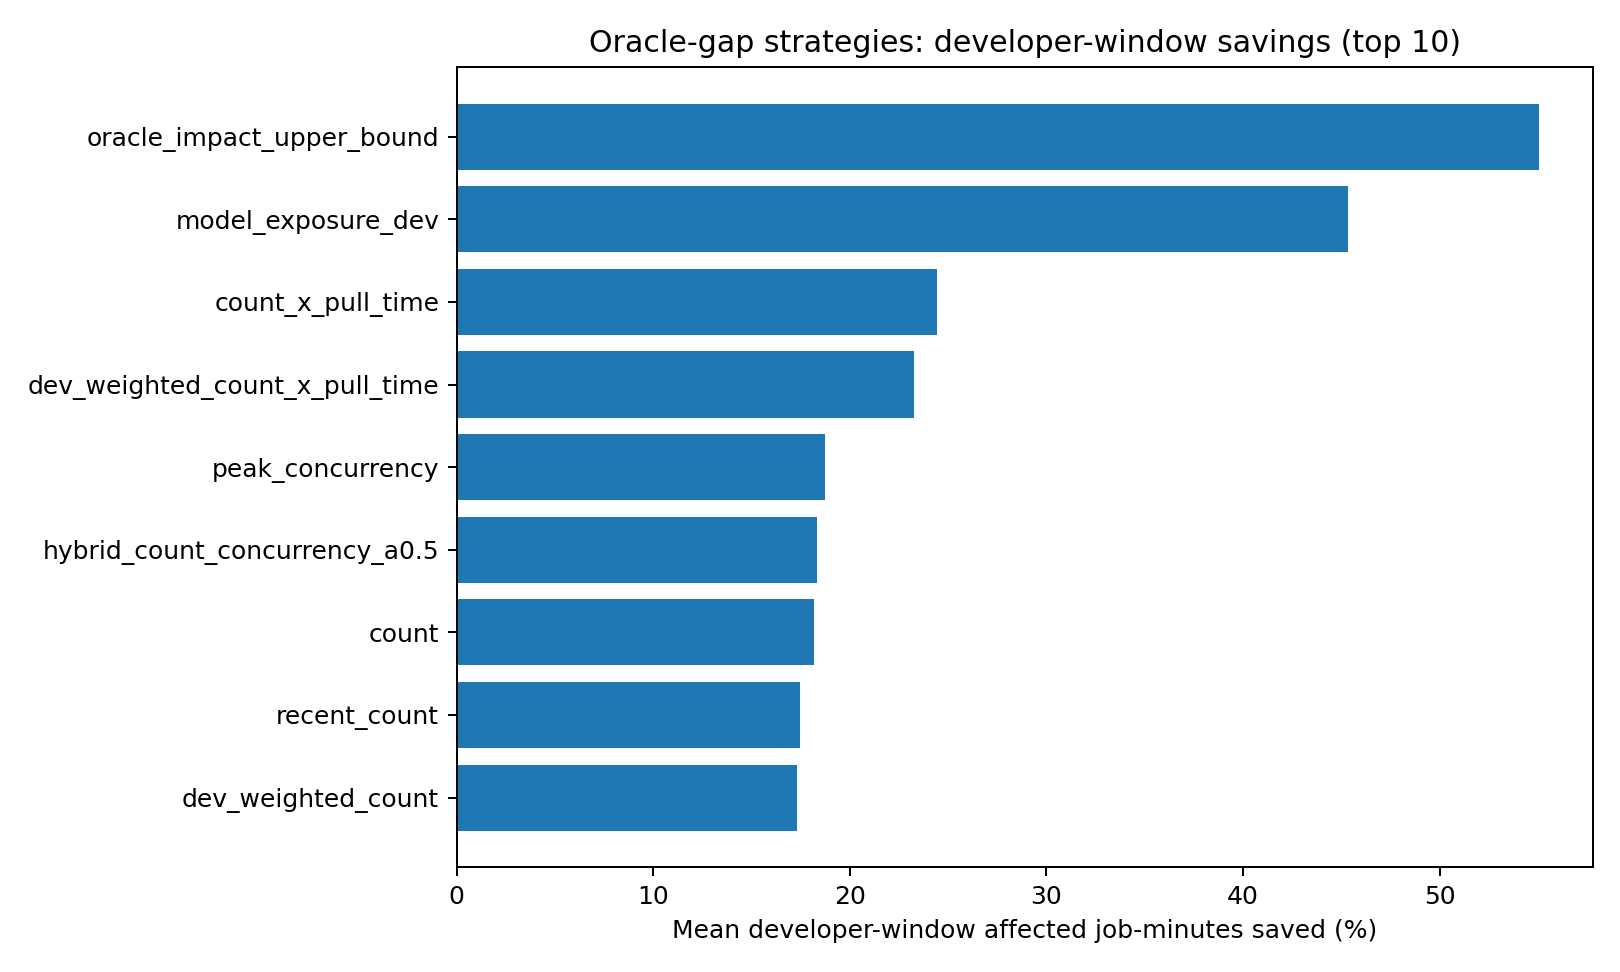
\includegraphics[width=0.92\linewidth]{figures/oracle_gap_dev_window_savings_top10.png}
\caption{Mean developer-window affected job-minutes saved by top-10 discovery strategy across 20 synthetic oracle-gap replay runs. Usage-only strategies cluster around 17--19\% developer-window savings. Adding pull-time information improves the ranking, and the model-aware exposure score closes most of the gap to the oracle upper bound.}
\label{fig:synthetic-oracle-gap-dev-savings}
\end{figure}

The oracle-gap replay suggests a practical maturity ladder for discovery. Usage-only controller strategies such as total usage and peak concurrency are safe first implementations because they require only Prometheus image observations. Adding measured image-availability time \(\hat{p}_I\) improves the approximation because high-impact images are not necessarily the most frequent. The strongest non-oracle result in this synthetic benchmark is the model-aware exposure score, which combines expected developer-window demand, estimated remaining cold-node fraction, and measured pull cost. In a real cluster, this requires additional measurement from Kubernetes Events, kubelet image-pull metrics, or replay-derived startup-delay estimates.


\section{Conclusion}

Node rotation in a dedicated Kubernetes CI node pool resets node-local image caches for important CI images. This paper models the resulting delay as developer-facing cold-node exposure: jobs are affected when they are scheduled onto nodes where the required OCI image \(I\) is not yet available for their startup path.

The single-image model is the foundation. It shows why affected jobs and newly warmed nodes are different quantities. Under burst or rolling-concurrency behavior, multiple jobs can wait on the same cold node before image availability changes, while that node becomes warm only once. This distinction matters because CI systems often create many jobs close together during fan-out stages or high-activity developer feedback windows.

The portfolio view turns the model into an operational prioritization problem. Real CI systems use many images, and the highest-frequency image is not always the image with the largest waiting contribution. Prewarming should therefore be evaluated by which images should already be warm on which eligible nodes before developer-facing CI load arrives.

The practical contribution is a real-cluster benchmark methodology. Cluster image-availability measurements estimate \(p_I\) from kubelet metrics, Kubernetes Events, or startup-delay proxies. GitLab Kubernetes executor replay then estimates how often those image-availability costs appear in CI workloads. Together, they can estimate affected jobs, newly warmed nodes, affected job-minutes, pipeline critical-path delay, and the impact of alternative cache policies.

Prewarming and cluster-local mirroring address different parts of the startup path. Prewarming reduces the probability that a developer-facing job hits a cold node. A cluster-local mirror such as Spegel can reduce \(p_I\) for remaining cold pulls when peer nodes already have useful layers. The most useful production evaluation is therefore a policy comparison: no prewarming, paced prewarming, cluster-local mirroring, and combined approaches replayed against real CI workload traces.

The synthetic evaluator included with this work is only a methodology sanity check. It demonstrates the type of comparison the replay method can produce, but it is not evidence of universal savings and does not replace production measurements. Production validation should combine measured image-availability distributions with real GitLab Kubernetes executor replay after node rotation, then compare modeled exposure with observed pipeline feedback delay.

\begin{thebibliography}{99}

\bibitem{gitlabjobs}
GitLab. \emph{CI/CD jobs}. \url{https://docs.gitlab.com/ci/jobs/}. Accessed 2026-06-09.

\bibitem{gitlabpipelines}
GitLab. \emph{CI/CD pipelines}. \url{https://docs.gitlab.com/ci/pipelines/}. Accessed 2026-06-09.

\bibitem{kubernetespods}
Kubernetes Documentation. \emph{Pods}. \url{https://kubernetes.io/docs/concepts/workloads/pods/}. Accessed 2026-06-09.

\bibitem{kubernetesnodes}
Kubernetes Documentation. \emph{Nodes}. \url{https://kubernetes.io/docs/concepts/architecture/nodes/}. Accessed 2026-06-09.

\bibitem{kubernetesimages}
Kubernetes Documentation. \emph{Images}. \url{https://kubernetes.io/docs/concepts/containers/images/}. Accessed 2026-06-09.

\bibitem{kubeletconfig}
Kubernetes Documentation. \emph{Kubelet Configuration (v1beta1)}. \url{https://kubernetes.io/docs/reference/config-api/kubelet-config.v1beta1/}. Accessed 2026-06-09.

\bibitem{schedulerconfig}
Kubernetes Documentation. \emph{Scheduler Configuration}. \url{https://kubernetes.io/docs/reference/scheduling/config/}. Accessed 2026-06-09.

\bibitem{kubernetesdaemonset}
Kubernetes Documentation. \emph{DaemonSet}. \url{https://kubernetes.io/docs/concepts/workloads/controllers/daemonset/}. Accessed 2026-06-09.

\bibitem{ociimage}
Open Container Initiative. \emph{OCI Image Format Specification}. \url{https://specs.opencontainers.org/image-spec/}. Accessed 2026-06-09.

\bibitem{ociimageconfig}
Open Container Initiative. \emph{OCI Image Configuration}. \url{https://specs.opencontainers.org/image-spec/config/}. Accessed 2026-06-09.

\bibitem{ocidistribution}
Open Container Initiative. \emph{OCI Distribution Specification}. \url{https://specs.opencontainers.org/distribution-spec/}. Accessed 2026-06-09.

\bibitem{containerdcri}
containerd. \emph{CRI Plugin Config Guide}. \url{https://containerd.io/docs/2.1/cri/config/}. Accessed 2026-06-09.

\bibitem{kubernetesimagepuller}
che-incubator. \emph{Kubernetes Image Puller}. \url{https://github.com/che-incubator/kubernetes-image-puller}. Accessed 2026-06-09.

\bibitem{kubefledged}
senthilrch. \emph{kube-fledged: a Kubernetes operator for creating and managing a cache of container images}. \url{https://github.com/senthilrch/kube-fledged}. Accessed 2026-06-09.

\bibitem{drop}
corewire. \emph{Drop Image Caching Operator}. \url{https://github.com/corewire/drop}. Accessed 2026-06-09.

\bibitem{dropdiscovery}
corewire. \emph{Drop Image Caching Operator Documentation: Discovery}. \url{https://corewire.github.io/drop/docs/discovery/}. Accessed 2026-06-17.

\bibitem{stargzsnapshotter}
containerd. \emph{Stargz Snapshotter: Fast container image distribution plugin with lazy pulling}. \url{https://github.com/containerd/stargz-snapshotter}. Accessed 2026-06-09.

\bibitem{sociintro}
AWS. \emph{Introducing Seekable OCI for lazy loading container images}. \url{https://aws.amazon.com/about-aws/whats-new/2022/09/introducing-seekable-oci-lazy-loading-container-images/}. Accessed 2026-06-09.

\bibitem{socifargate}
AWS Containers Blog. \emph{Under the hood: Lazy Loading Container Images with Seekable OCI and AWS Fargate}. \url{https://aws.amazon.com/blogs/containers/under-the-hood-lazy-loading-container-images-with-seekable-oci-and-aws-fargate/}. Accessed 2026-06-09.


\bibitem{clusterapimachinedeployment}
Cluster API. \emph{MachineDeployment Controller}. \url{https://main.cluster-api.sigs.k8s.io/developer/core/controllers/machine-deployment}. Accessed 2026-06-09.

\bibitem{prometheusoverview}
Prometheus Documentation. \emph{Overview}. \url{https://prometheus.io/docs/introduction/overview/}. Accessed 2026-06-09.

\bibitem{mimiroverview}
Grafana Labs. \emph{Grafana Mimir documentation}. \url{https://grafana.com/docs/mimir/latest/}. Accessed 2026-06-09.

\bibitem{kubestatemetrics}
Kubernetes Documentation. \emph{Metrics for Kubernetes Object States}. \url{https://kubernetes.io/docs/concepts/cluster-administration/kube-state-metrics/}. Accessed 2026-06-09.

\bibitem{kubeletmetrics}
Kubernetes Documentation. \emph{Metrics Reference}. \url{https://kubernetes.io/docs/reference/instrumentation/metrics/}. Accessed 2026-06-26.


\bibitem{clusterapioverview}
Cluster API. \emph{Kubernetes Cluster API}. \url{https://cluster-api.sigs.k8s.io/}. Accessed 2026-06-10.

\bibitem{clusterapiconcepts}
Cluster API. \emph{Concepts: Machine Immutability}. \url{https://cluster-api.sigs.k8s.io/user/concepts.html}. Accessed 2026-06-10.


\bibitem{spegel}
Spegel Project. \emph{Spegel: Stateless cluster local OCI registry mirror}. \url{https://spegel.dev/}. Accessed 2026-06-21.

\bibitem{spegelarchitecture}
Spegel Project. \emph{Spegel Architecture}. \url{https://spegel.dev/docs/architecture/}. Accessed 2026-06-21.

\end{thebibliography}

\end{document}
